
\documentclass[oneside]{ausarbeitung}
\bibliography{latexlit}


% ----------------------------------------------------------------------

\begin{document}

%--- Sprachauswahl
% Erlaubte Werte:
%   \selectlanguage{english}
%   \selectlanguage{ngerman}
\selectlanguage{ngerman}

%--- Art der Arbeit
% Erlaubte Werte:
%   \Praxissemesterbericht
%   \Projektbericht
%   \Bachelorarbeit
%   \Seminararbeit
%   \Masterarbeit

\Projektbericht

%--- Studiengang:
% Erlaubte Werte:
%   \Informatik
%   \Elektronik
%   \DataScience
\Informatik

\title{Visualisierung von MongoDB Datenbanken}

\author{Max Winter}
\matrikelnr{80559}

%--- Ist der Erstbetreuer (\examinerA) an der Hochschule ein Professor?
% Erlaubte Werte:
%   \examinerIsAProfessortrue   % Ja
%   \examinerIsAProfessorfalse  % Nein
\examinerIsAProfessortrue   % Ja

%--- Betreuer
\examinerA{Prof.~Dr.~Gregor Grambow}
%\examinerB{Prof.~Dr.~Ulrich~Klauck}

%--- Einreichungsdatum
\date{01. Dezember 2016}

%--- Angaben zur Firma
% Auskommentieren, wenn die Arbeit nicht bei einer ext. Firma gemacht wurde.
%\companyname{Beispielfirma}
%\industrialsector{Beispielbranche}
%\department{Beispielabteilung}
%\companystreet{Beispielstr. 1}
%\companycity{12345 Musterstadt}

%--- Angaben zum Betreuer bei dieser Firma
%\advisorname{Name des Betreuers}
%\advisorphone{(01234) 567-890}
%\advisoremail{name@company.xxx}

%--- Titelseite Anzeigen
\maketitle
\cleardoublepage

%---
\pagenumbering{roman}
\setcounter{page}{1}

%--- Firmendaten Anzeigen
% Auskommentieren, wenn die Arbeit nicht bei einer ext. Firma gemacht wurde.
%\makeworkplace
%\cleardoublepage

%--- Eidesstattliche Erklärung anzeigen
\makeaffirmation
\cleardoublepage

%---
\begin{abstract}

    \iffalse
    Ziel der Kurzfassung ist es, einen (eiligen) Leser zu informieren, so 
    dass dieser entscheiden kann, ob der Bericht für ihn hilfreich ist oder 
    nicht (neudeutsch: Management Summary). Die Kurzfassung gibt daher eine 
    kurze Darstellung

    \begin{itemize}
    \item des in der Arbeit angegangenen Problems
    \item der verwendeten Methode(n)
    \item des in der Arbeit erzielten Fortschritts.
    \end{itemize}

    Dabei sollte nicht auf die Struktur der Arbeit eingegangen werden, also 
    Kapitel~\ref{cha:grundlagen} etc. denn die Kurzfassung soll ja gerade 
    das Wichtigste der Arbeit vermitteln, ohne dass diese gelesen werden muss.
    Eine Kapitelbezogene Darstellung sollte sich in Kapitel~%
    \ref{cha:einleitung} unter Vorgehen befinden.

    Länge: Maximal 1 Seite.
    \fi

    In diesem Bericht geht es um die Entwicklung eines Visualisierungstools für MongoDB Datenbanken.
    Ziel dieses Tools ist es, aus den Dokumenten und Collections einer MongoDB Datenbank Schemas zu extrahieren, welche daraufhin anschaulich visualisiert werden.
    Dieses Tool ist Teil eines größeren Datenbank Toolkits, weshalb in der Entwicklung großen Wert auf Modulatität und Erweiterbarkeit gelegt wird.

    Das MongoDB Visualisierungstool besteht aus einem React Frontend und einem Flask Backend, welche über HTTP miteinander kommunizieren.
    Die Aufgabe des Backends ist es, sich mit einer MongoDB Datenbank zu verbinden.
    Diese Datenbank wird bei erfolgreicher Verbindung analysiert und das Ergebnis der Analyse an das Frontend zurückgegeben.
    Das Frontend visualisiert diese Daten daraufhin in Form von Tabellen.
    
    Das Erarbeiten dieses Tools wird in diesem Bericht von der Problemstellung über die Planung und Entwicklung bis hin zu der Auslieferung erläutert.
    In der Einleitung wird zunächst die Bedeutung von MongoDB und die Wichtigkeit dieses Tools herausgearbeitet.
    Im Kapitel Grundlagen werden daraufhin einige Technologien vorgestellt, die für die Lösung des Problems benötigt werden.
    Welche Anforderungen das Tool erfüllen muss, um als Erfolg gewertet werden zu können, wird im Kapitel Problemanalyse herausgearbeitet.
    Im Lösungskonzept werden zunächst die bestehenden Analyse- und Visualisierungstools für MongoDB analysiert, um den Nutzen und die Besonderheit des MongoDB Visualisierungstools herauszufinden.
    Daraufhin wird ermittelt, mit welchen Tools sich die in der Problemanalyse erarbeiteten Anforderungen am besten erfüllen lassen.
    Anschließend wird geplant, wie die konkrete Umsetzung aussehen soll.
    Im Backend geschiet dies vor allem anhand von UML-Diagrammen, im Frontend anhand von Wireframes.
    In der Implementierung wird die Umsetzung dieses Lösungskonzepts in Python und JavaScript dokumentiert.
    Abschließend wird noch die Auslieferung der Lösung, sowie die Evaluierung der Ergebnisse und einen Ausblick auf die weitere Entwicklung des Database Toolkits präsentiert.
    
    
\end{abstract}

%-----------------------------------------------------------------------
\cleardoublepage
\tableofcontents

%---
\listoffigures

%---
\listoftables

%---
\lstlistoflistings

%---
\listofabbreviations
\begin{acronym}[Bsp.]  % Längstes Kürzel in der nachfolgenden
                       % Liste um die Breite der Spalte für die
                       % Abkürzungen zu bestimmen.

%% Eintrag: \acro{Referenzname}[Kürzel]{Langform}
%% Im Text wird die Abkürzung dann mit \ac{Referenzname} benutzt.
\acro{rup}[RUP]{Rational Unified Process}
\acro{sql}[SQL]{Structured Query Language}
\acro{http}[HTTP]{Hypertext Transfer Protocol}
\acro{api}[API]{Application Programming Interface}
\acro{rest}[REST]{Representational State Transfer}
\acro{json}[JSON]{JavaScript Object Notation}
\acro{url}[URL]{Uniform Resource Locator}
\acro{ui}[UI]{User Interface}   
\acro{uri}[URI]{Uniform Resource Identifier}
\acro{uuid}[UUID]{Universally Unique Identifier}
\acro{dto}[DTO]{Data Transfer Object}
\acro{ddl}[DDL]{Data Definition Language}
\acro{dml}[DML]{Data Manipulation Language}
\acro{xml}[XML]{Extensible Markup Language}
\acro{jaxrs}[JAX-RS]{Jakarta RESTful Web Services}
\acro{pojo}[POJO]{Plain Old Java Object}
\end{acronym}
%---


\cleardoublepage
\pagenumbering{arabic}
\setcounter{page}{1}

% ----------------------------------------------------------------------
\chapter{Einleitung}
\label{cha:einleitung}
\iffalse
Die Einleitung dient dazu, beim Leser Interesse für die Inhalte 
Praxissemesterberichts zu wecken, die behandelten Probleme aufzuzeigen 
und die zu ihrer Lösung entwickelten Konzepte zu beschreiben.
\fi

\section{Motivation}
\label{sec:motivation}

\iffalse
In der Motivation wird dargestellt, welche Bedeutung die im 
Praxissemester zu entwickelnden Lösungen für das betreuende Unternehmen 
haben. Es wird beispielsweise aufzeigt, in welches Produkt sie eingehen, 
welcher Ablauf verbessert werden soll etc.
\fi

Für einen Entwickler, der mit einer Datenbank arbeitet, ist es wichtig zu wissen, wie diese Datenbank aussieht, was für Abhängigkeiten es gibt, und ob die Implementierung auch wirklich der Planung entspricht.
Aus diesem Grund werden Visualisierungs- und Analysetools für Datenbanken benötigt.
MongoDB hat sich in den letzten Jahren zu einem der wichtigsten Datenbanksysteme entwickelt, da aufgrund immer größerer werdenden Datenmengen die Vorteile von NoSQL-Datenbanken für immer mehr Anwendungen überwiegen.
~\autocite{db-engines:mongodb}
Da MongoDB keine relationale Datenbank ist, können herkömmliche Visualisierungs- und Analysetools, die für SQL entwickelt wurden, nicht verwendet werden.
Für MongoDB gibt es zwar Visualisierungstools, wie Beispielsweise MongoDB Charts und MongoDB Compass, die meisten davon visualisieren aber die Daten in der Datenbank, und nicht die Struktur und das Schema der Dokumente in der Datenbank.
~\autocite{knowi:mongo_vis_tools}
Die Daten selbst können jedoch sehr vielzahlig sein, was ein vollständiges Überblicken der Datenbank schwierig bis unmöglich macht.
Auß diesem Grund soll das Ziel dieser Arbeit sein, solch ein Visualisierungstool zu entwickeln.

\section{Problemstellung und -abgrenzung}
\label{sec:problemstellung}

\iffalse
Die Problemstellung dient dazu, das zu lösende Problem klar zu 
definieren und abzugrenzen. Der Praktikant soll ein klares Verständnis 
des zu lösenden Problems haben. Insbesondere soll auch verhindert 
werden, dass zu viele Probleme gleichzeitig angegangen werden. Eine 
Negativabgrenzung verhindert, dass beim Leser später nicht erfüllte 
Erwartungen geweckt werden.
\fi

Es soll ein MongoDB Visualisierungstool entwickelt werden, welches eine MongoDB Datenbank analysiert und auswertet.
Daraus sollen Schemas extrahiert und visualisiert werden.
Das Visualisieren der konkreten Daten in der MongoDB Datenbank ist nicht Teil des Problems.

\section{Vorangegangene Arbeit}
\label{sec:vorangegangene_arbeit}

Das MongoDB Visualisierungstool soll in eine vorangegangene Arbeit integriert werden.
In dieser vorangegangenen Arbeit wurde ein Entity-Relationship Modellierungstool entwickelt.
Einer der Ziele dieses Modellierungstools war es, die Anwendung möglichst modular zu gestalten, damit das Modellierungstool langfristig zu einem umfassenden Datenbank-Toolkit erweitert werden kann.
~\autocite{ruttmann:projektarbeit}
Ein Hauptfokus des MongoDB Visualisierungstools liegt deshalb darauf, diese Modularität beizubehalten und gegebenenfalls weiter zu verbessern.

\section{Ziel der Arbeit}
\label{sec:ziel}

Ziel dieses Projekts ist es, ein Visualisierungstool für MongoDB Datenbanken zu entwickeln, welches die Dokumente einer Datenbank analysiert und auswertet.
Daraus sollen Schemas abgeleitet werden, welche anschließend visualisiert werden.
Dies erleichtert es den Entwicklern der Datenbanken, die Strukturen und Abhängigkeiten in ihren Datenbanken zu verstehen und zu verbessern.
Dafür soll eine Backendanwendung zur Verbindung und Analyse von MongoDb Datenbanken entwickelt werden, sowie ein Webfrontend für die Visualisierung der analysierten Daten.
Das Visualisierungstool soll dabei in die vorangegangene Arbeit integriert werden und die Gesamtlösung dabei modular halten.

Um Datenbanken analysieren zu können, muss es möglich sein, sich mit diesen zu verbinden.
Dies erfordert einerseits eine Nutzeroberfläche, über die der Nutzer die Verbindungsdaten eingeben kann.
Andererseits erfordert dies die Verbindung mit der Datenbank selbst über eine geeignete MongoDB Schnittstelle im Backend.
Die Dokumente der Datenbank müssen anschließend in möglichst kurzer Zeit analysiert werden, um aus ihnen Schemas zu extrahieren.
Diese Schemas müssen dann in einem Frontend übersichtlich und visuell ansprechend angezeigt werden.
Dafür werden hauptsächlich 2 Ansichten benötigt:
Einerseits wird eine Übersicht über alle Collections benötigt, in welcher  für jede Collection das meistverwendete Schema angezeigt werden soll.
Andererseits wird für jede Collection eine Detailansicht benötigt, welche alle Schema-Variationen in einer Collection sowie  weitere Details und Daten anzeigt.


\iffalse
\section{Vorgehen}
\label{sec:vorgehen}

Nachdem mit Problemstellung und Ziel gewissermaßen Anfangs- und Endpunkt 
des Praktikums beschrieben sind, wird hier der zur Erreichung des Ziels 
eingeschlagene Weg vorgestellt. Dazu werden typischerweise die folgenden 
Kapitel und ihr Beitrag zur Erreichung des Ziels der Arbeit kurz 
beschrieben. Die folgenden Kapitel sind ein – möglicher – Aufbau, 
Abweichungen können durchaus notwendig sein. Zur Darstellung des 
Vorgehens ist eine grafische Darstellung sinnvoll, bei der die einzelnen 
Lösungsschritte und ihr Zusammenhang dargestellt werden. Ein Beispiel 
hierfür findet sich in Abbildung \ref{fig:1}.
\fi


% ---
\chapter{Grundlagen}
\label{cha:grundlagen}
\iffalse
In diesem Kapitel das für das Praktikum relevante Grundlagenwissen 
dargestellt. Der Praktikant soll hierzu das ihm durch Vorlesungen 
bekannte, bzw. durch Recherchen vertiefte theoretische Wissen 
darstellen, das für die Lösung der im Praktikum gestellten Probleme 
notwendig ist.

Dabei ist darauf zu achten, nur solche Inhalte in das Grundlagenkapitel 
aufzunehmen, die später auch verwendet werden (Problembezogenheit). 
Ebenso ist auf eine ausreichend tiefe und vollständige Darstellung der 
Grundlagen zu achten.

Für die Erstellung des Literaturverzeichnisses 
wird das Werkzeug JabRef\autocite{JabRef:JabRef} verwendet. 

Sie können aber auch das Werkzeug Citavi\autocite{SAS:Citavi} benutzen
und dort nach \textsc{Bib}\TeX{} exportieren.
\fi

Im folgenden werden einige Tools und Technologien beschrieben, welche für die Entwicklung des MongoDB Visualisierungstools sowie für die Nachfolgenden Kapitel eine wichtige Rolle spielen.

\section{HTTP}
\label{sec:http}

\ac{http} ist ein Protokoll, welches benutzt wird, um über das Internet zu kommunizieren.
Hauptsächlich wird \ac{http} für die Kommunikation zwischen einem Webbrowser und einem Webserver genutzt.
In \ac{http} wird mittels Nachrichten kommuniziert.
Es wird erst ein Request vom Client abgesetzt, der daraufhin von dem Server mit einer Response beantwortet wird.
Nachrichten bestehen aus einem Header und einem Body.
Der Body enthält den Inhalt der Nachricht.
Der Header enthält Meta-Daten über einen Request, wie beispielsweise die angefragten Ressourcen und Datentypen des Body.

\section{REST API}
\label{sec:rest}

Ein \ac{api} ist eine Schnittstelle, über die von außen mit einem Programm interagiert werden kann.
\ac{rest} ist ein Protokoll, welches die Kommunikation über HTTP spezifiziert.
\ac{rest} sieht ein Backend vor, welches Resourcen beinhaltet.
Ein Client kann über die gängigen \nameref{sec:http} Operationen mit diesen Resourcen interagieren.
Jede Resource hat eine global eindeutige ID und wird meist durch \ac{json} oder \ac{xml} repräsentiert.
In Java wird ein \ac{rest}ful Webservice für gewöhnlich mit \ac{jaxrs} umgesetzt.
~\autocite{schiesser:javaEE7}

\section{SQL}
\label{sec:sql}

Die \ac{sql} ist eine Datenbanksprache für relationale Datenbanken.
In \ac{sql} werden die Daten in Tabellen organisiert, die ein festes Schema definieren.
Man kann \ac{sql} in 2 Teile aufteilen:
Die \ac{ddl} definiert den Aufbau des Schemas.
Mit ihr können Datenbankobjekte erzeugt und gelöscht werden.
Zur \ac{ddl} gehören unter anderem die Befehle CREATE, ALTER, DROP und TRUNCATE\@.
Mit der \ac{dml} können Daten manipuliert, also eingefügt, geändert, gelesen und gelöscht werden.
Die Befehle hierfür lauten SELECT, INSERT, UPDATE, DELETE, MERGE und noch weitere.
~\autocite{schicker:datenbanken}

\section{JSON}
\label{sec:json}

\ac{json} ist ein Format zum Datenaustausch.
\ac{json} basiert auf der Syntax von JavaScript Objekten, ist jedoch unabhängig von der Programmiersprache einsetzbar.
Vorteile von \ac{json} sind die einfache Lesbarkeit für Menschen und das einfache parsen und generieren für Maschinen.
~\autocite{json:json}
In JSON gibt es unter anderem folgende Datentypen:

\begin{figure}[H]
    \begin{minipage}[t]{0.45\textwidth}
        \flushleft\textbf{Object} ist ein Set aus Key/Value Paaren.
        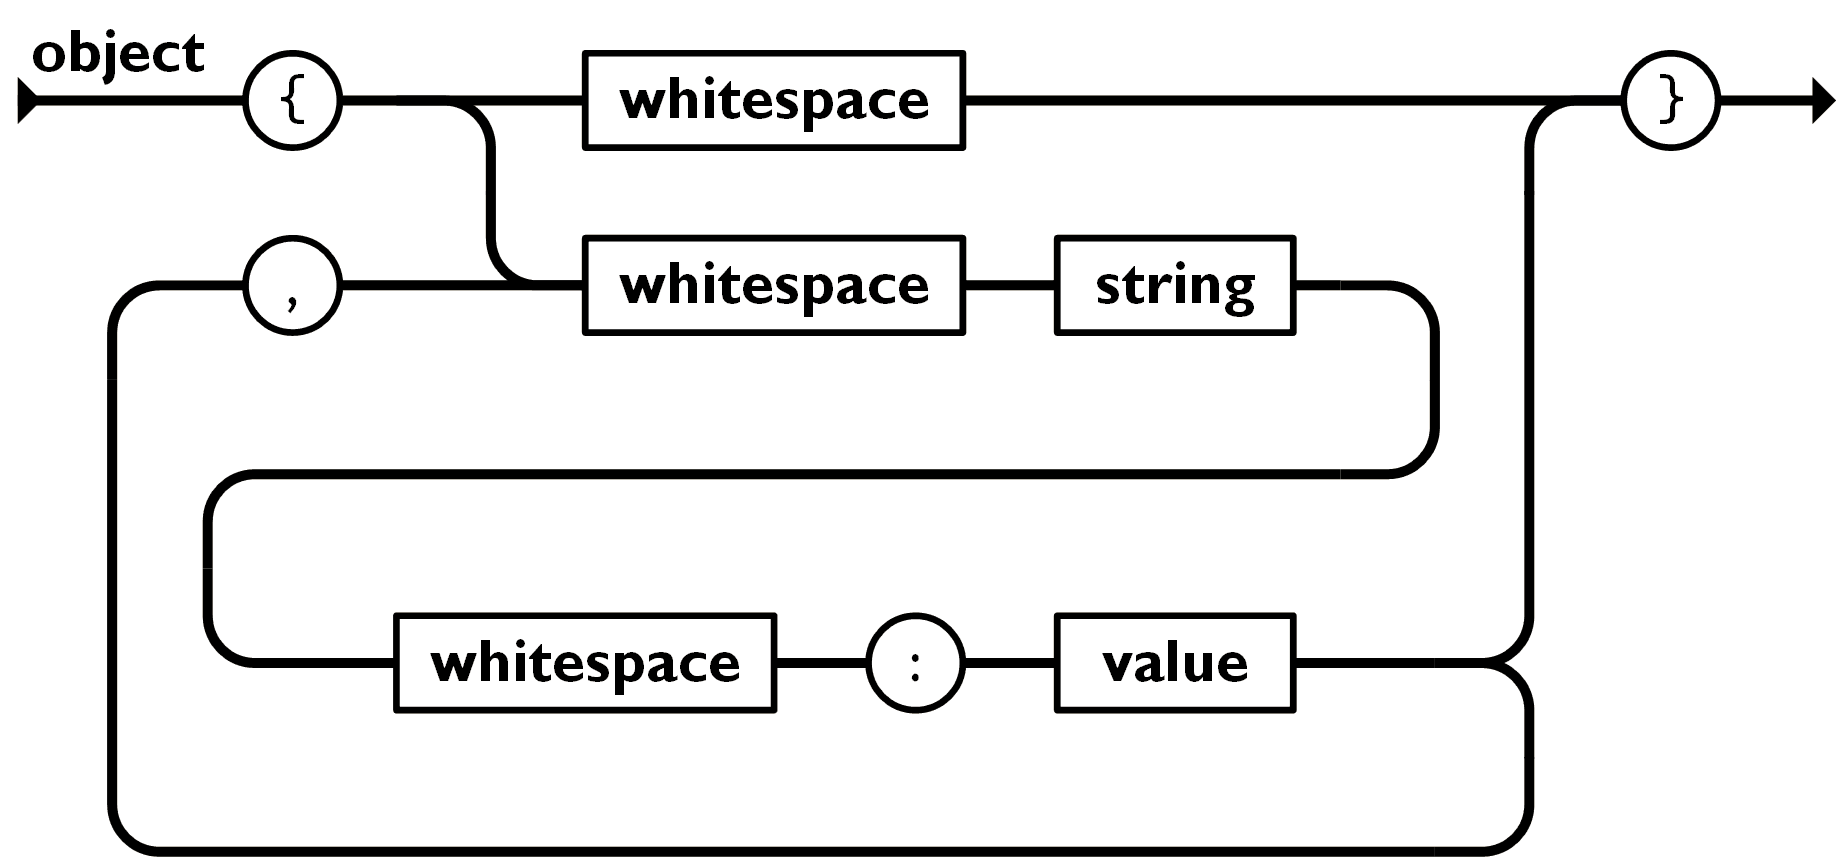
\includegraphics[width=0.9\textwidth]{images/json_object}
        \caption{JSON Object}
        \label{fig:json_object}
    \end{minipage}\hfill
    \begin{minipage}[t]{0.45\textwidth}
        \flushleft\textbf{Array} ist eine geordnete Liste von Values.
        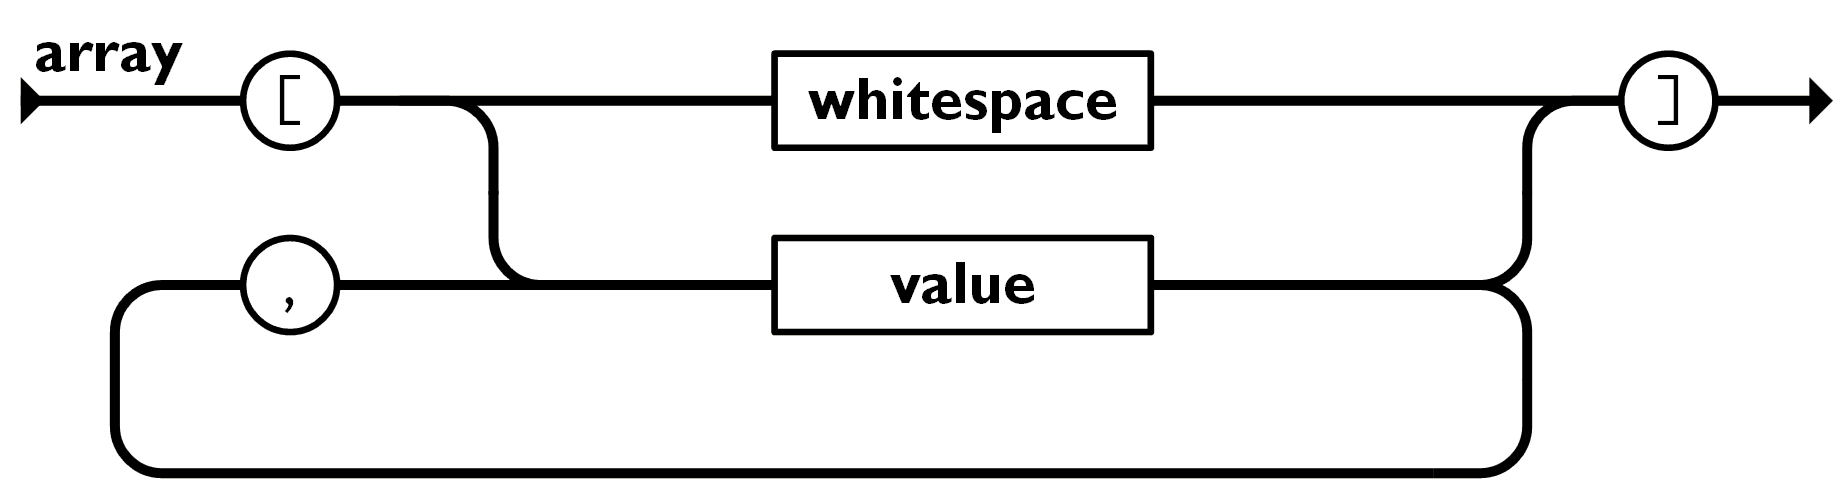
\includegraphics[width=0.9\textwidth]{images/json_array}
        \caption{JSON Array}
        \label{fig:json_array}
    \end{minipage}\hfill
\end{figure}
\begin{figure}[H]
    \begin{minipage}[t]{0.45\textwidth}
        \textbf{Value} kann ein String, eine Zahl, ein Boolean, ein Objekt, ein Array oder null sein.
        Dabei können beliebig viele Values ineinander verschachtelt sein.
        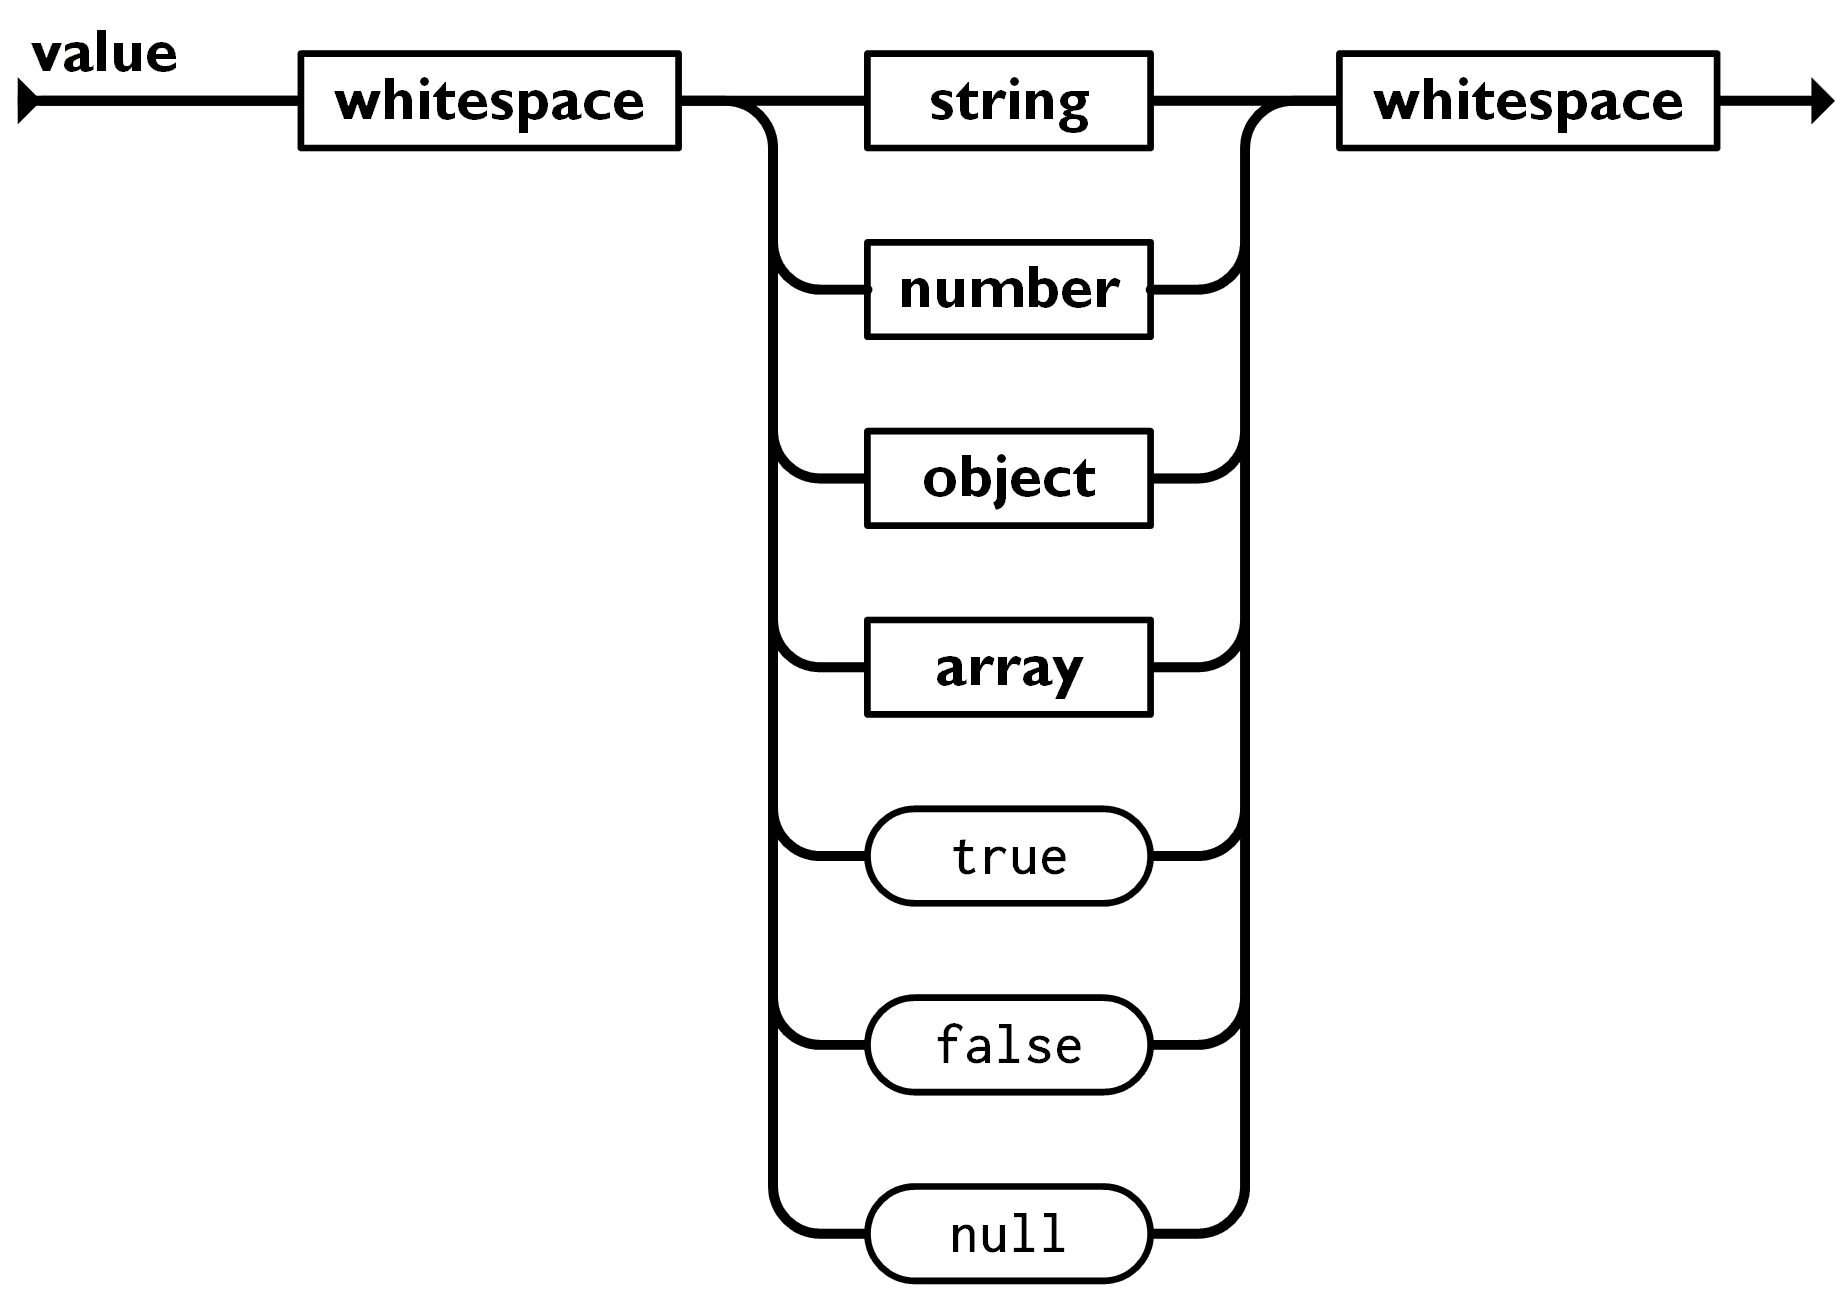
\includegraphics[width=0.9\textwidth]{images/json_value}
        \caption{JSON Value}
        \label{fig:json_value}
    \end{minipage}\hfill
    \begin{minipage}[t]{0.45\textwidth}
        \flushleft\textbf{String} ist eine Sequenz aus Unicode Buchstaben.
        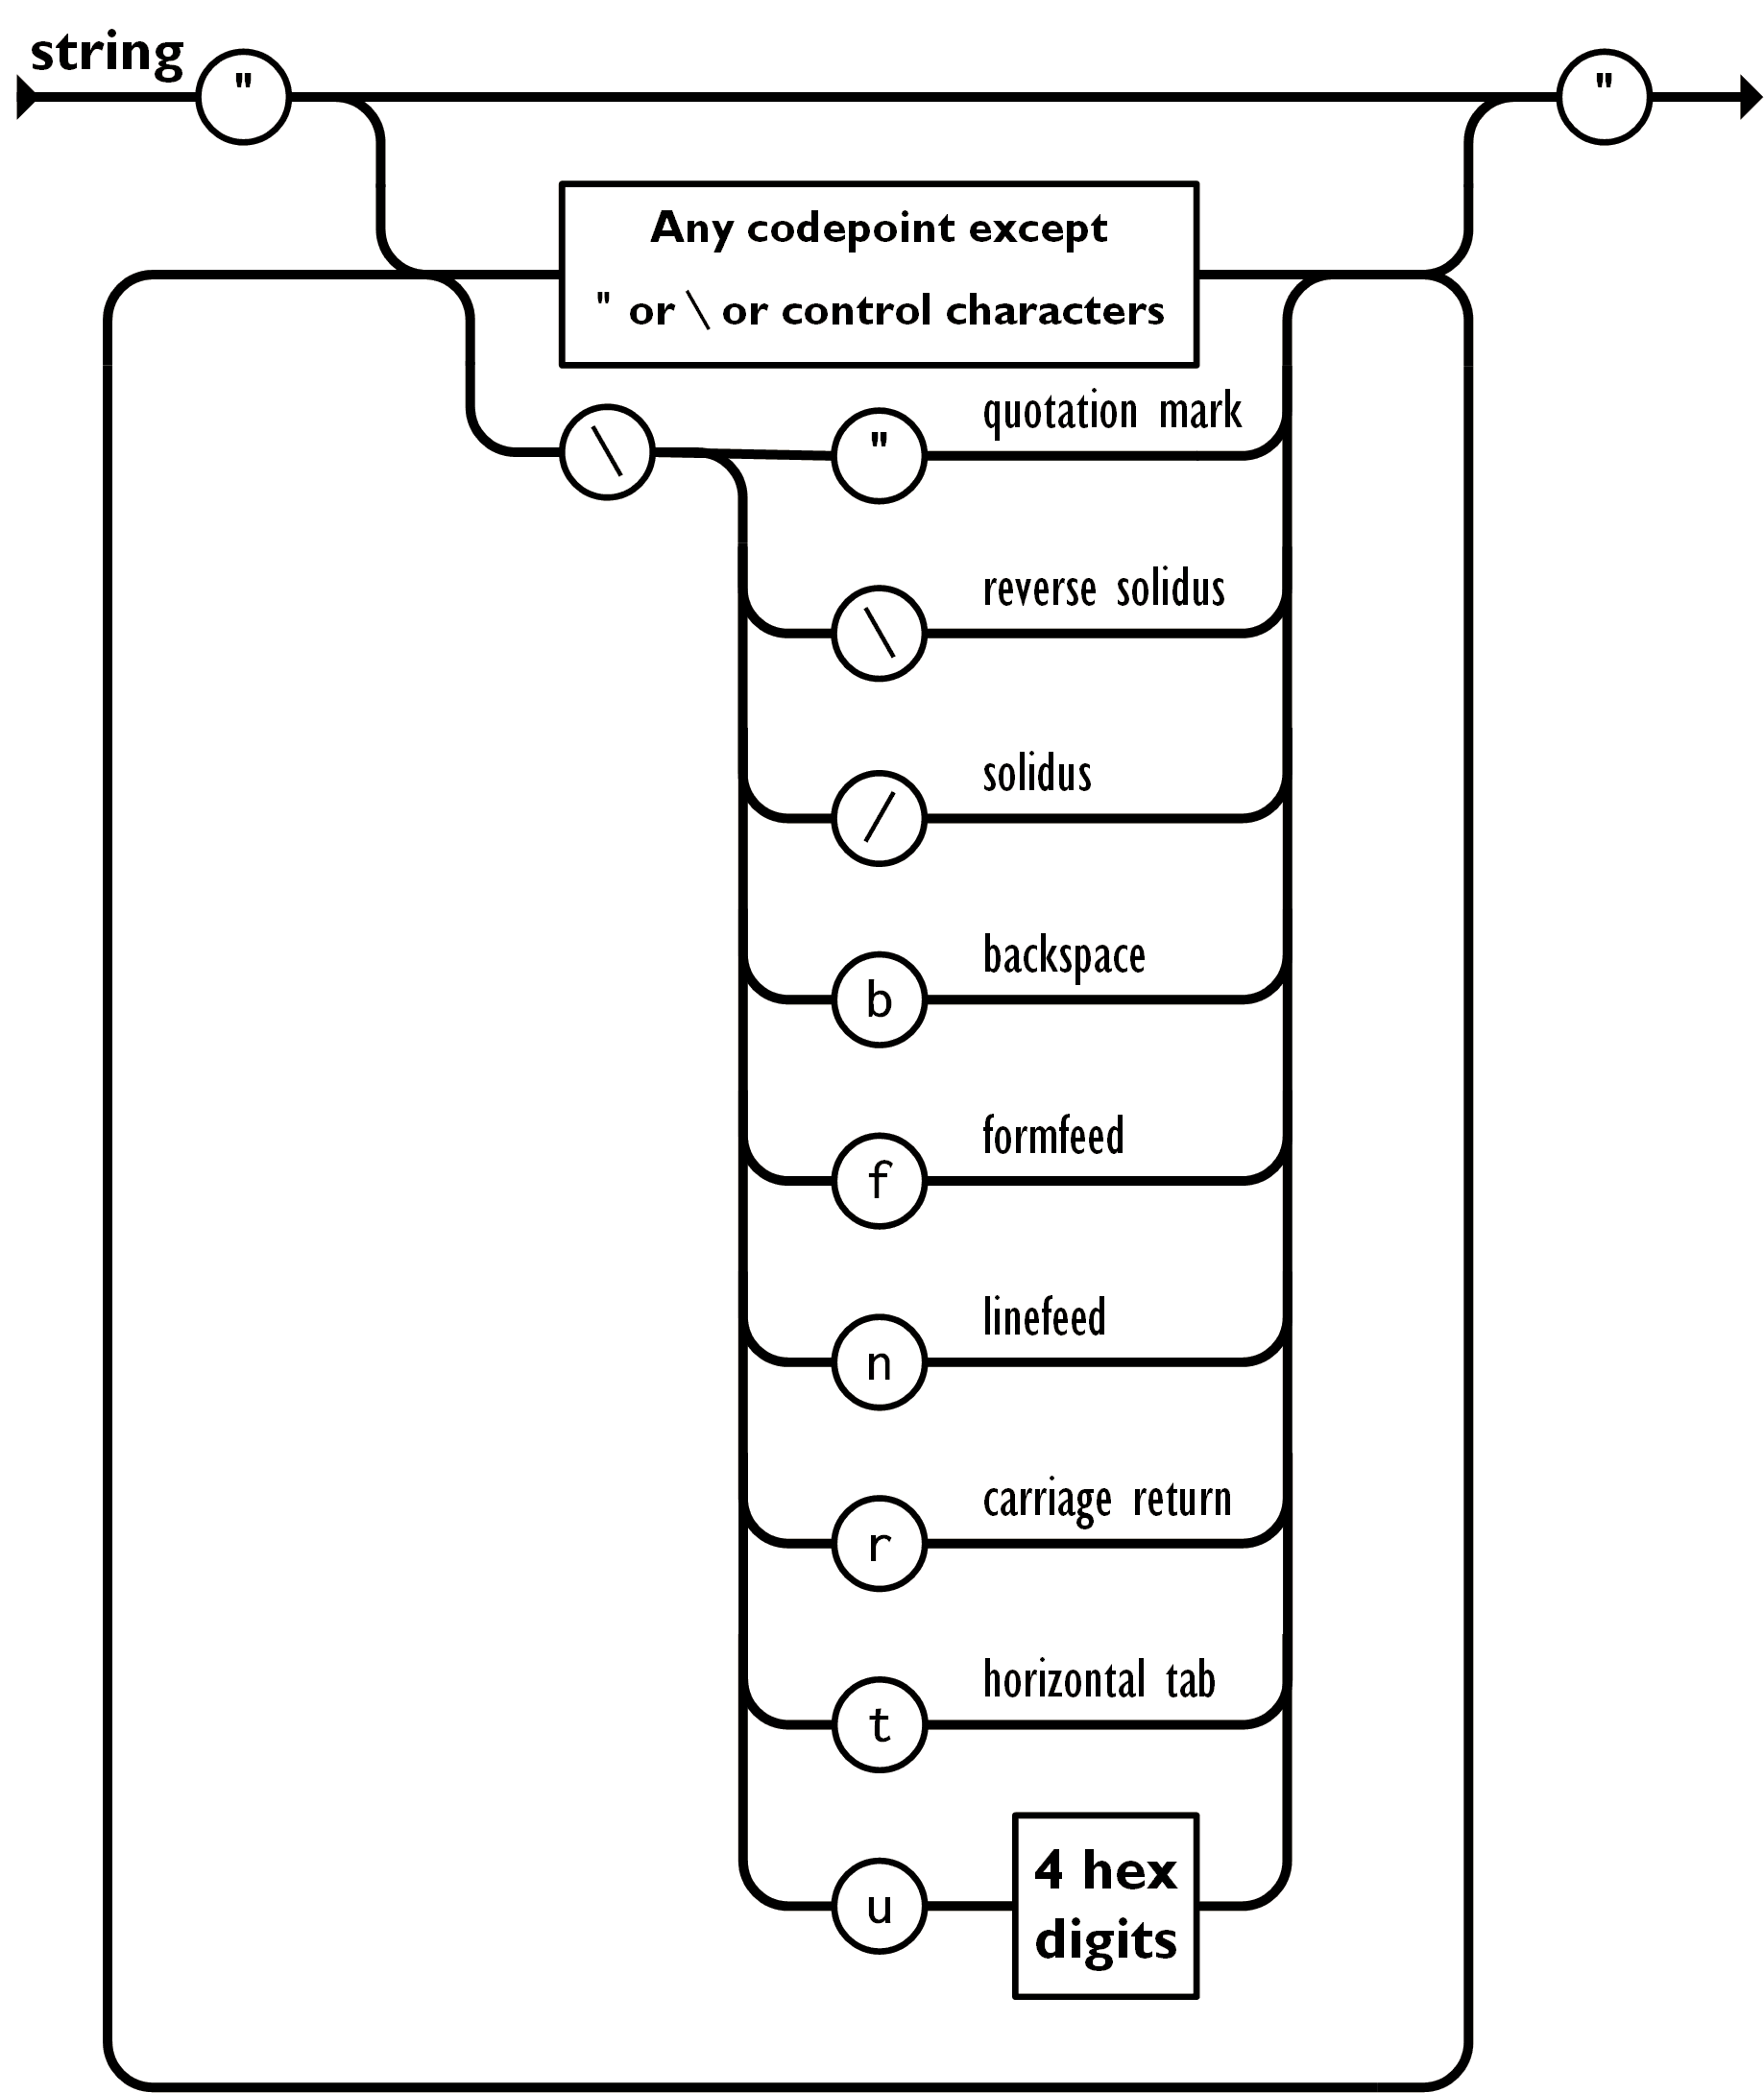
\includegraphics[width=0.9\textwidth]{images/json_string}
        \caption{JSON String}
        \label{fig:json_string}
    \end{minipage}\hfill
\end{figure}
\begin{figure}[H]
    \begin{minipage}[t]{0.45\textwidth}
        \textbf{Number} ist eine Zahl.
        Number kann sowohl eine Gleitkommazahl als auch eine Ganzzahl sein und kann positiv sowie negativ sein.
        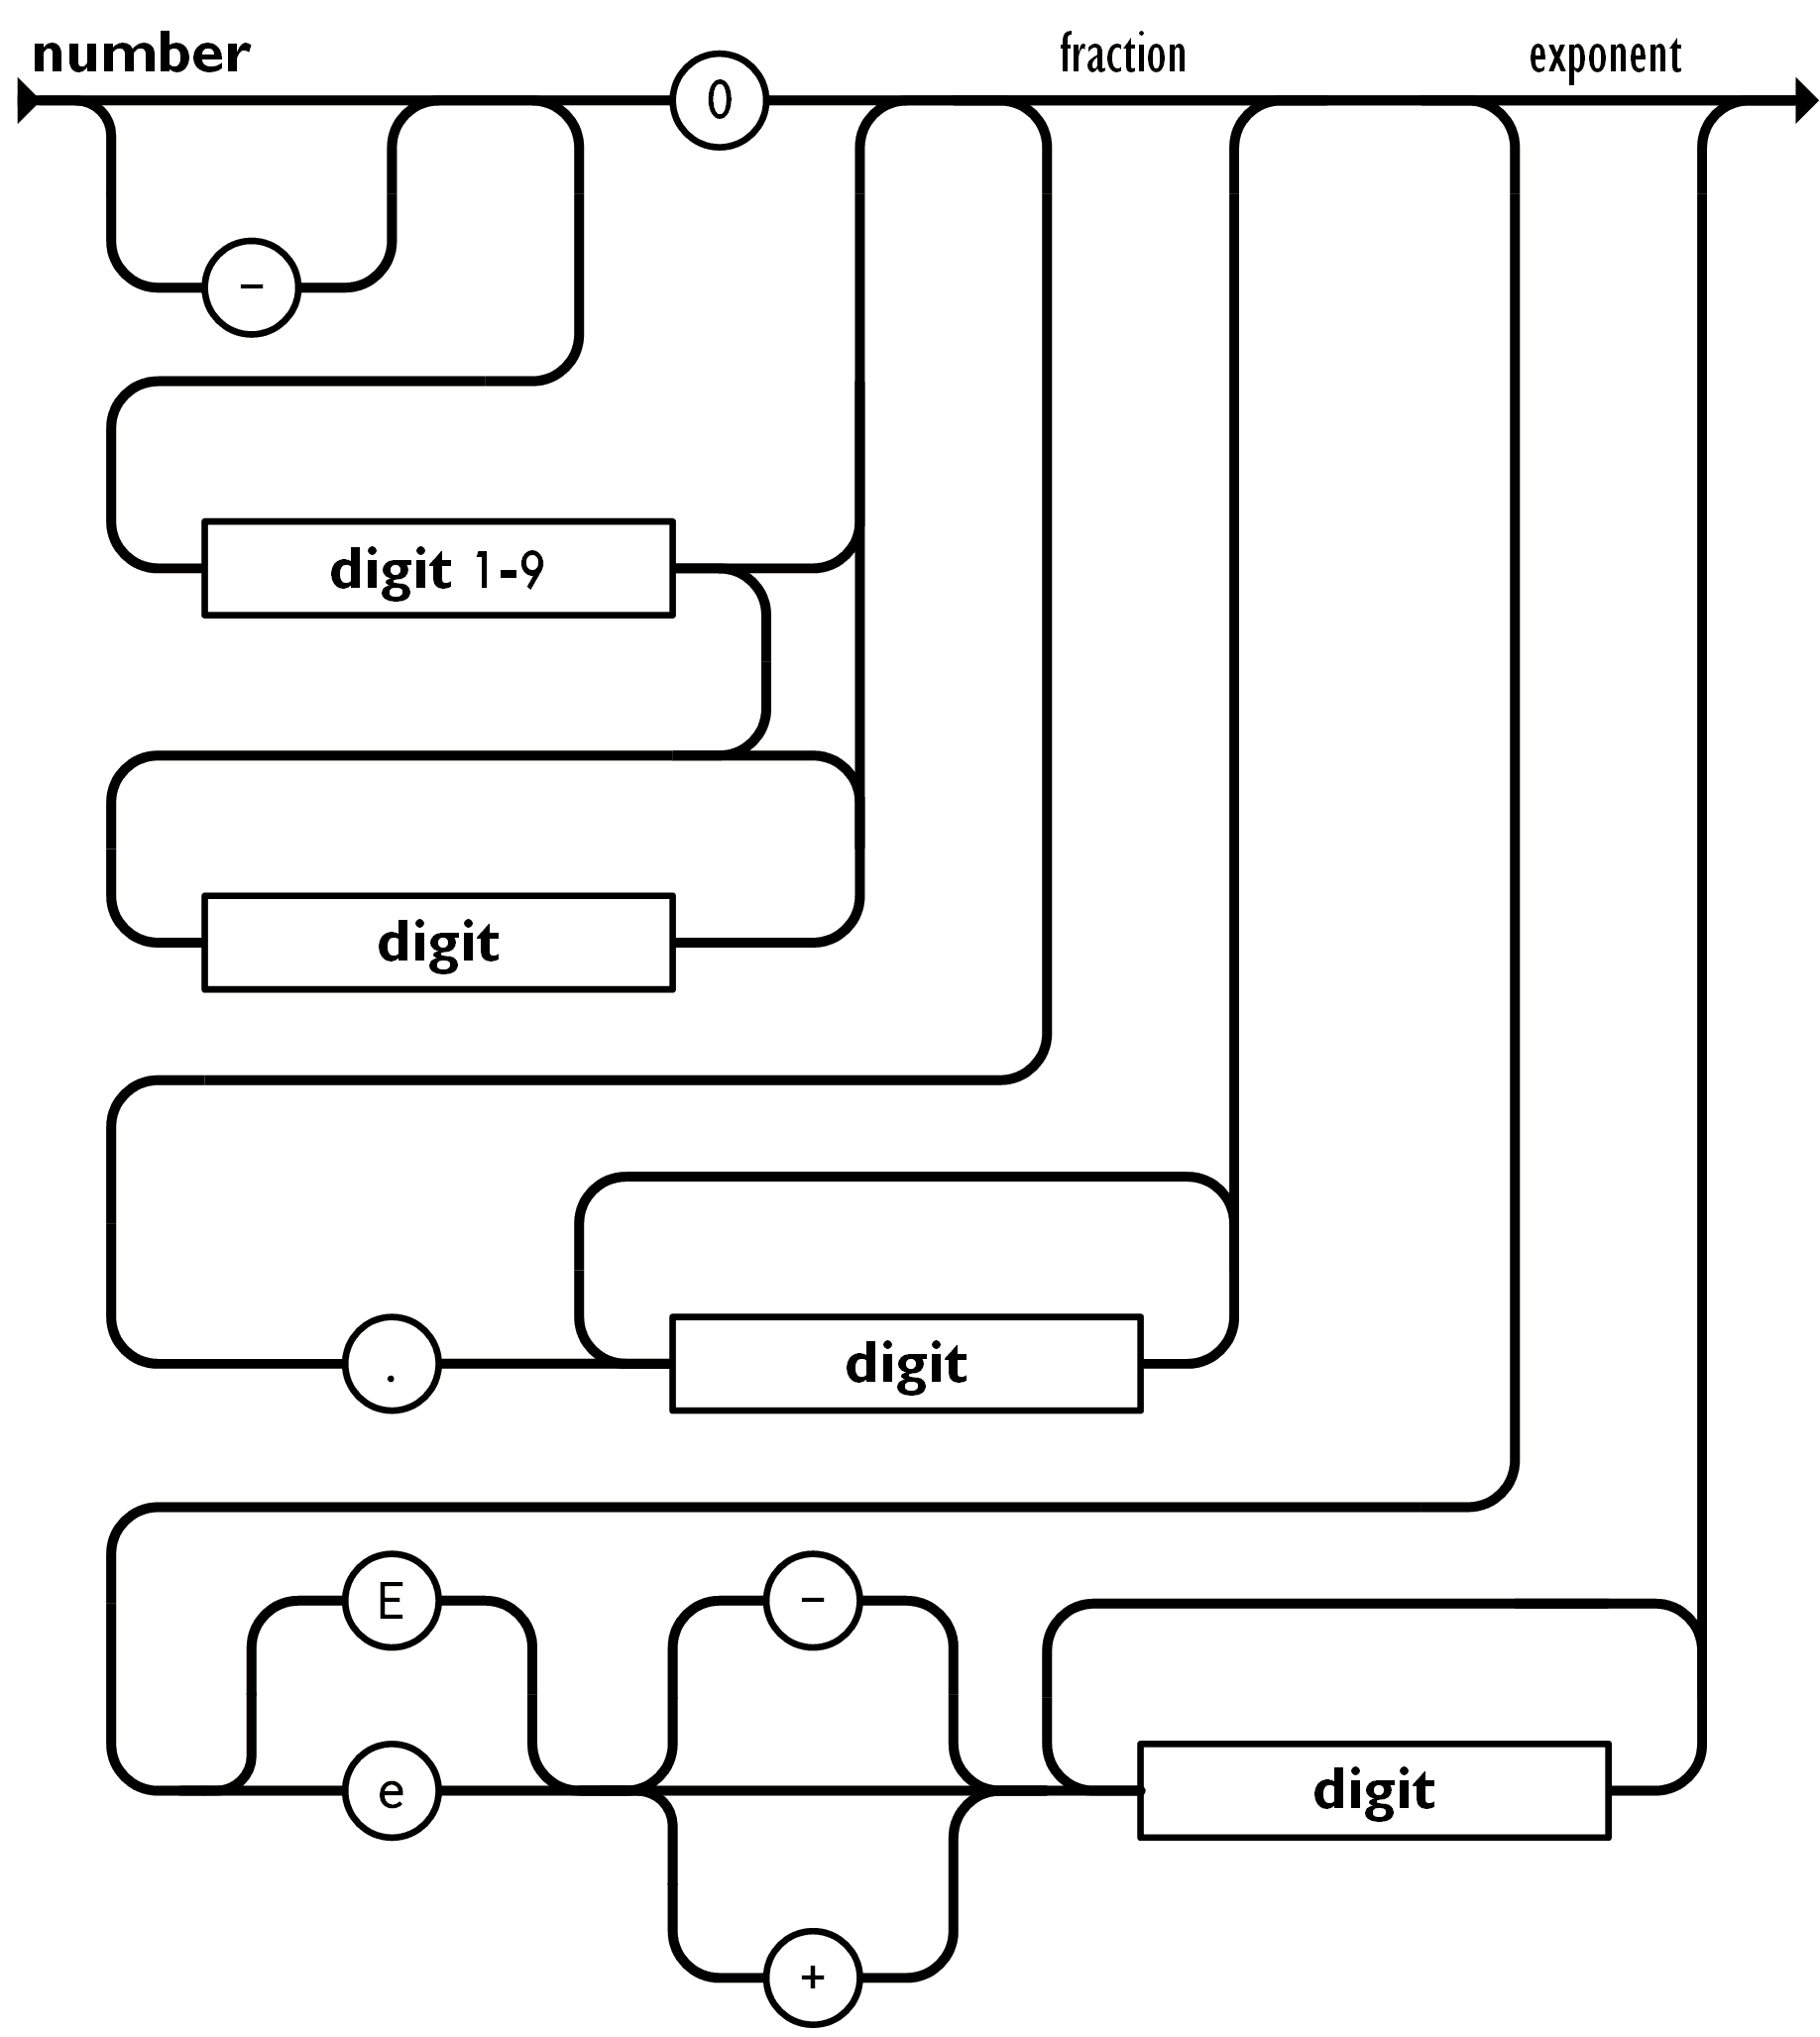
\includegraphics[width=0.9\textwidth]{images/json_number}
        \caption{JSON Number}
        \label{fig:json_number}
    \end{minipage}\hfill
\end{figure}

\section{MongoDB}
\label{sec:mongodb}

MongoDB ist eine Dokument-orientierte Datenbank. 
In Dokument-orientierten Datenbanken wird das aus SQL bekannte Konzept von Reihen durch Dokumente ersetzt.
Dokumente haben im Gegensatz zu Reihen in Tabellen kein fixes Schema, welches sie erfüllen müssen, sondern sind sehr flexibel.
Grundsätzlich bestehen Dokumente aus Key - Value Paaren, welche in einer JSON-Ähnlichen Struktur gespeichert werden.
Dokumente können, wie auch in JSON, ineinander verschachtelt sein, was hierarchische Strukturen und dadurch Denormalisierung ermöglicht.
Die Dokumente werden in Collections organisiert.
Eine Collection entspricht in SQL einer Tabelle ohne das fixe Schema.
Diese Collections befinden sich wiederum in Datenbanken.
Eine MongoDB Instanz kann mehrere voneinander unabhängige Datenbanken beinhalten.
Man kann sich mit der MongoShell mit einer MongoDB Instanz verbinden, um mit der Mongo Query Language oder mit JavaScript die Instanz administrieren und Daten manipulieren zu können.
~\autocite{bradshaw:mongodb}

\section{Python}
\label{sec:python}

Python ist eine objektorientierte high-level Programmiersprache, die besonderen Wert auf Lesbarkeit legt.
Variablen in Python werden dynamisch typisiert.
Das bedeutet, dass eine Variable in Python keinen festen Typ hat, sondern dieser dynamisch über den ihr zugewiesenen Wert bestimmt wird.
Python ist keine kompilierte, sondern eine interpretierte Programmiersprache.
Diese Eigenschaften machen Python zu der idealen Sprache für das Schreiben von Skripten, sowie für Anwendungen, die schnell und simpel entwickelt werden sollen.
PIP ist ein in Python integrierter Paketmanager, der das installieren von Packages erleichtert.
Der Python Interpreter ist in C geschrieben, weshalb man die Funktionalität des Interpreters durch C-Programme erweitern kann, um beispielsweise laufzeitkritische Funktionen in C auszuführen.
~\autocite{van:python}

\section{Flask}
\label{sec:flask}

Flask ist ein minimalistisches Open-Source Web Framework für Python.
In Flask sind ein paar wenige Kernpakete vorinstalliert, welche für ein minimales Backend benötigt werden.
Alles weitere muss der Nutzer selbst über PIP installieren.
~\autocite{grindberg:flask}
Durch diesen minimalistischen Ansatz ist Flask sehr flexibel einsetzbar.
Flask ist beispielsweise mit SQL oder NoSQL Datenbanken, aber auch ganz ohne Datenbanken einsetzbar.

\section{JavaScript}
\label{sec:js}

JavaScript ist eine High-Level Programmiersprache, die just-in-time kompiliert wird.
JavaScript ist besonders bekannt als Skriptsprache für Webseiten, wird aber auch für Backendanwendungen, Automatisierungsaufgaben und vieles mehr verwendet.
Die Besonderheit von JavaScript gegenüber anderen Sprachen ist eine vollständige native Kompatibilität und Integration in HTML und CSS.
~\autocite{javascript:javascript}
Die Pakete in JavaScript werden mittels dem Paketmanager NPM verwaltet.

\section{React}
\label{sec:react}

React ist eine JavaScript Bibliothek zum Bauen von Benutzeroberflächen.
React ist Komponentenbasiert.
Das bedeutet, dass React aus einzelnen Komponenten bestehen, die ihren eigenen State haben und die zusammengesetzt ein komplexes \ac{ui} bilden.
~\autocite{banks:react}


\subsection{Redux Store}
\label{sub:redux}

Redux ist ein State Container für JavaScript Apps, der es ermöglicht, States nicht mehr in den einzelnen React Komponenten, sondern in einem zentralen Container zu speichern.
~\autocite{freecodecamp:redux}
Dadurch können States wiederhergestellt werden, nachdem eine Komponente geschlossen und wieder geöffnet wurde.
Außerdem erleichtert Redux es, State Änderungen in Komponenten nachzuvollziehen.

\iffalse
\subsection{Axios}
\label{sub:axios}

Axios ist ein HTTP-Client für JavaScript.
Mithilfe von Axios Können HTTP-Requests versendet und die Responses von diesen verarbeitet werden.
\fi

\section{Docker Container}
\label{sec:docker}

Ein Container ist eine virtuelle Umgebung, die, ähnlich wie eine virtuelle Maschine, eine Anwendung in eine isolierte Umgebung verpackt.
Jedoch wird im Gegensatz zu virtuellen Maschinen nicht das ganze Betriebssystem virtualisiert, sondern nur einzelne Anwendungen.
Dadurch ist ein Container deutlich schlanker als eine virtuelle Maschine.
Container können als sogenannte Images auf verschiedenen Systemen ausgeliefert werden und dabei aufgrund der Isolierung unabhängig vom System zuverlässig funktionieren.
Docker ist eine weit verbreitete Open-Source Software, welche das Container-Prinzip implementiert.
~\autocite{devInsider:container}

\section{Nginx}
\label{sec:nginx}

Nginx, ausgesprochen Engine X, ist ein Open-Source Web Server.
In Nginx sind einige Features für das Hosten von Webservern integriert, wie beispielsweise Load Balancing, Reverse Proxies, Web Sockets, Mail Server und vieles mehr.
Dabei unterstütz Nginx alle gängigen Betriebssysteme, wie Windows, Windows Server, MacOS und Linux.
Die Konfiguration in Nginx erfolgt über Konfigurationsdateien.
Die Nutzung von Nginx als Webserver nimmt jedes Jahr weiter zu im Vergleich zum Kompetitoren wie Apache.
Im Januar 2023 liefen 21,20\% der meistgenutzten Seiten über Nginx.
~\autocite{nginx:nginx}

\section{Microservice Architektur}
\label{sec:microservices}

Die Microservice Architektur ist eine Architektur, bei der das Endprodukt aus einer Sammlung einzelner Services besteht.
Diese Services sind an sich voneinander unabhängig auslieferbar und sind nur lose gekoppelt.
Jeder Service wird von einem einzelnen kleinen Team entwickelt und muss ohne großen Aufwand testbar und wartbar sein.
~\autocite{richardson:microservices}


%---
\chapter{Problemanalyse}
\label{cha:problemanalyse}
\iffalse
Die Analyse des zu lösenden Problems ist Grundlage für jedes 
ingenieurmäßige Vorgehen. Daher soll in diesem Kapitel das zu lösenden 
Problem auf Basis des im Grundlagenkapitel aufbereiteten Wissens 
analysiert werden. Hierzu ist insbesondere notwendig zu klären, wie sich 
das Gesamtproblem in Teilprobleme zerlegen lässt und welche 
Abhängigkeiten zwischen diesen bestehen.

Bei Software-Projekten befindet sich an dieser Stelle typischerweise die 
Anforderungsanalyse des \ac{rup}.

Anforderungen:
\begin{itemize}
    \item modular
    \item erweiterbar
    \item performant
\end{itemize}

\fi

An das MongoDB Visualisierungstool gibt es eine Reihe von Anforderungen, welche erfüllt werden müssen, damit das Projekt als Erfolg gewertet werden kann.
Diese werden im Nachfolgenden nach Frontend und Backend getrennt analysiert.

\section{Anforderungen an das Frontend}
\label{sec:anf_frontend}

Das Resultat des Projekts soll eine Gesamtlösung sein, die aus dem bestehenden ER Modellierungstool und dem MongoDB Visualisierungstool besteht. 
Diese Gesamtlösung soll flexibel durch weitere Anwendungen und Funktionalitäten erweitert werden können.
Das Frontend des ER-Modellierungstools besteht aus einer React Webapp.
Deshalb muss das Frontend der Gesamtlösung ebenfalls in einer gemeinsamen Webapp ausgeliefert werden (\nameref{itm:fa1}).
Diese Webapp muss in der Paketstruktur sowie in den verwendeten Komponenten modular sein (\nameref{itm:fa2}).
Ohne diese Modularität wäre die Erweiterbarkeit des Frontends nicht gegeben.
Um auf die einzelnen Tools der Gesamtlösung zugreifen zu können, wird ein Startbildschirm benötigt, von welchem aus man die Tools starten kann (\nameref{itm:fa3}). 

Da das MongoDB Visualisierungstool ein relativ kleines Tool ohne großen Funktionsumfang ist, sind die meisten Nutzer nicht bereit, erst ein Handbuch für die Benutzung der Anwendung zu lesen.
Aus diesem Grund muss die Anwendeung intuitiv benutzbar sein.
Das bedeutet, dass alle Funktionen der Anwendung selbsterklärend, oder in der Anwendung selbst ausreichend beschrieben sein müssen (\nameref{itm:fa4}).
Dies erfordert auch, dass sich alle Frontend-Anwendungen der Gesamtlösung gleich benutzen lassen und ein einheitliches Design verwenden, da dies sonst den Arbeitsfluss und dadurch die intuitive Bedienung behindert (\nameref{itm:fa5}).

MongoDB Dokumente können beliebig groß und beliebig verschachtelt sein.
Ein Dokument kann eingebettete Dokumente, sowie Arrays in beliebiger Tiefe ineinander geschachtelt haben.
Damit die Visualisierung großer Dokumente trotzdem einen Mehrwert hat, müssen diese unabhängig von der Größe übersichtlich und verständlich sein.
Aus diesem Grund ist eine übersichtliche Darstellung der Schemata sehr wichtig (\nameref{itm:fa6}).

Die Dokumente in einer Collection müssen nicht zwangsläufig das gleiche Schema haben.
Diese Schema Abweichungen können verschiedene Ursachen haben:
Das Schema kann einige optionale Felder haben, welche in manchen Dokumenten nicht gesetzt sind.
Es könnte sich aber auch um verschiedene Versionen eines Schemas handeln, das sich im Laufe der Entwicklung gewandelt hat.
Es könnte sich bei den Abweichungen aber auch um Fehler in der Implementierung handeln.
Für einen Entwickler kann es deshalb hilfreich sein, einen Überblick über alle Variationen in einer Collection zu haben.
Aus diesem Grund soll das MongoDB Visualisierungstool für jede Collection eine Detailansicht haben, welche diese Variationen visualisiert.
Der Unterschied in diesen Variationen kann vor allem bei großen Dokumenten unter Umständen nicht direkt ersichtlich sein.
Aus diesem Grund müssen diese Abweichungen vom Hauptschema deutlich hervorgehoben werden.(\nameref{itm:fa7})

\section{Anforderungen an das Backend}
\label{sec:anf_backend}

Das MongoDB Visualisierungstool muss auch sehr große MongoDB Datenbanken analysieren können.
Vor allem bei großen Datenbanken ist ein Visualisierungstool besonders hilfreich, da große Datenmengen sehr schwer überschaubar sind.
Die Analyse sollte jedoch nicht länger als ein paar Sekunden dauern, da dies den Arbeitsfluss der Benutzer unterbrechen würde.
Ein Entwickler sollte während der Arbeit an der Datenbank das Visualisierungstool schnell starten können, um ihn bei der Analyse der Datenbank zu unterstützen.
Deshalb müssen die Datenbanken möglichst performant analysiert werden.
Die Laufzeit der Analyse sollte 10 Sekunden nicht überschreiten (\nameref{itm:ba1}).

Die Webapp kann potenziell von beliebig vielen Personen gleichzeitig benutzt werden.
Dies bedeutet, dass das Backend des MongoDB Visualisierungstools mehrere Anfragen gleichzeitig abarbeiten können muss.
Deshalb müssen mehrere MongoDB Datenbanken gleichzeitig verbunden und analysiert werden könnnen (\nameref{itm:ba2}).

\cleardoublepage

\section{Übersicht über die Anforderungen}
\label{sec:anf_uebersicht}

\textbf{Frontend:}

\begin{description}
    \item[\textbf{FA1}\label{itm:fa1}] Gemeinsame Webapp aller Anwendungen der Gesamtlösung
    \item[\textbf{FA2}\label{itm:fa2}] Modularität
    \item[\textbf{FA3}\label{itm:fa3}] Startbildschirm
    \item[\textbf{FA4}\label{itm:fa4}] Intuitive Benutzbarkeit
    \item[\textbf{FA5}\label{itm:fa5}] Einheitliches Design und Layout
    \item[\textbf{FA6}\label{itm:fa6}] Übersichtliche Darstellung der Schemata
    \item[\textbf{FA7}\label{itm:fa7}] Visualisierung der Schema-Variationen in einer Collection
\end{description}

\textbf{Backend:}

\begin{description}
    \item[\textbf{BA1}\label{itm:ba1}] Analyse der Datenbanken in unter 10 Sekunden
    \item[\textbf{BA2}\label{itm:ba2}] Verbindung und Analyse mehrerer MongoDB Datenbanken gleichzeitig
\end{description}



%---
\chapter{Lösungskonzept}
\label{cha:loesungskonzept}
\iffalse
Auf der Basis der im vorangegangenen Kapitel erstellten Problemanalyse 
und der im Grundlagenkapitel aufgearbeiteten theoretischen Kenntnisse 
wird ein Lösungskonzept erarbeitet.

Bei Software-Projekten entspricht dieses Kapitel typischerweise der 
Analyse \& Design-Phase des \ac{rup}. Typische Ergebnisse dieser Phase sind 
Klassendiagramme etc.
\fi

% TODO wo soll diese Sektion hin?
\section{Bestehende Visualisierungstools}
\label{sec:bestehende_visualisierungstools}

Es gibt bereits MongoDB Visualisierungtools auf dem Markt, jedoch erfüllt keines davon die zuvor definierten Anforderungen zu genüge:

\begin{itemize}
    \item \textbf{MongoDB Data Explorer} ist ein Tool, welches in MongoDB Atlas integriert ist.
        MongoDB Atlas ist ein Web-Tool zur verwaltung von MongoDB Datenbanken.
        Mittels dem MongoDB Data Explorer kann man die Dokumente, Collections und Indexe einer Datenbank anschauen, sowie die Daten mit CRUD Operationen verwalten.
        Jedoch bietet der MongoDB Data Explorer keine Möglichkeiten, die Schemas der Dokumente zu analysieren.
    \item \textbf{MongoDB Compass} ist eine Desktop Anwendung zur Analyse von MongoDB Datenbanken.
        MongoDB Compass besitzt ein Schema-Visualisierungstool.
        Dieses Schema-Visualisierungstool zeigt sehr genaue Daten zu jedem Feld an, ist jedoch nicht besonders übersichtlich, wenn man das gesamte Schema der Dokumente einer Collection analysieren will.
        Ebenfalls nicht gut ersichtlich in MongoDB Compass ist die Varianz im Schema zwischen den Dokumenten in einer Collection.
    \item \textbf{MongoDB Charts, Tableau, Qlik und Looker} sind Tools, die aus MongoDB Daten Graphen generieren und dadurch die Daten in einer MongoDB visualisieren können.
        Diese Tools konzentrieren sich jedoch alle auf die Visualisierung der Daten, nicht die Analyse und Visualisierung der Schemas der Dokumente.
\end{itemize}
~\autocite{knowi:mongo_vis_tools}

\section{Verwendete Technologien}
\label{sec:verwendete_technologien}

\subsection{Backend Technologien}
\label{sec:verwendete_technologien_backend}

Da die Analyse der MongoDB Dokumente sehr rechenintensiv ist, wird die Analyse in ein Backend ausgelagert.
Um den zuvor definierten Anforderungen gerecht zu werden, ist es wichtig, ein geeignetes Backend-Framwork auszuwählen.
Das Er Modellierungstool nutzt Java Spring als Backend-Framework.
Da man zum Teil Code von dem bestehenden Backend übernehmen könnte, bietet es sich deshalb an, in diesem Projekt ebenfalls Spring zu verwenden.

Für Spring gibt es eine MongoDB Implementierung namens Spring Data MongoDB.
Diese Implementierung ist jedoch dafür ausgelegt, \ac{pojo}s auf Dokumente zu mappen.
Im MongoDB Visualisierungstool sollen hingegen MongoDB Dokumente dynamisch eingelesen und analysiert werden.
Um ~\nameref{itm:a5} zu erfüllen, ist es desweiteren nötig, beliebig viele verschiedene Datenbanken gleichzeitig zu verbinden und zu analysieren.
Die Verbindung mit MongoDB Datenbanken Spring Data MongoDB erfolgt jedoch mit festgelegten Datenbanken, welche in der application.properties Datei definiert werden.
~\autocite{spring:spring-data-mongodb}
Deshalb ist die Spring Data MongoDB Bibliothek für diese Anwendung nicht geeignet.
Neben der Spring Data MongoDB Bibliothek gibt es auch noch einen anderen MognoDB Java Client, Java Sync.
Dieser funktioniert jedoch nicht zusammen mit dem Spring Framework.
Aus diesem Grund kann Spring sowie andere Java Backend Frameworks nicht genutzt werden.

Als alternatives Backend Framework mit REST API bietet sich Flask an.
Ein großer Vorteil von Flask ist, dass Flask sehr minimal ist und nur mit dem minimum an benötigten Bibliotheken vorkonfiguriert ist.
Spring ist im Gegensatz dazu ein sehr mächtiges Framework mit vielen Features, von denen in diesem Projekt aber nur sehr wenige gebraucht werden.
Ein weiterer Vorteil von Flask sowie von Python ist die Schlankheit des Codes.
In Python lässt sich meist die gleiche Funktionalität in weniger Code schreiben als in Java.
Dazu kommt, dass in Flask sehr viel weniger Boilerplate Code benötigt wird als in Spring.
Ein minimaler Endpunkt in Flask lässt sich bereits mit 2 Zeilen Code umsetzen.
Zudem ist die dynamische Typisierung in Python beim Auswerten der MongoDB Dokumente von Vorteil, da man im Voraus nicht weiß, welche Datentypen die Werte in den Dokumenten haben, und die dynamische Typisierung deshalb das Handling dieser Werte vereinfacht.
~\autocite{khoirom2020comparative}
Jedoch hat Flask nicht nur Vorteile gegenüber Spring:
Flask ist grundsätzlich deutlich unperformanter als Spring.
Dies liegt unter anderem daran, dass Python eine interpretierte Sprache ist, und Java eine kompilierte.
~\autocite{sverker:rest_comparison}
Dies widerspricht zunächst der Anforderung ~\nameref{itm:a3}.
Die Performance-Probleme lassen sich aber durch Multiprocessing ausgleichen.
Multiprocessing bedeutet, dass bestimmte Teile der Berechnung auf mehrere Threads im Prozessor aufgeteilt werden und dadurch parallell ausgeführt werden.
Python bietet eine simpel zu implementierende Lösung für Multiprocessing an, welche man bei der Analyse der Dokumente der MongoDB Datenbanken gut einsetzen kann.
Beispielsweise kann die Analyse jeder Collection von einem extra Thread ausgeführt werden.
Dadurch lässt sich die Anforderung ~\nameref{itm:a3} mit Flask erfüllen.

In Python gibt es die Bibliothek PyMongo, welche alle der genannten Nachteile von Spring Data MongoDB ausbessert:
Mit PyMongo kann man direkt im Code beliebig viele MongoDB Datenbanken parallel dynamisch einbinden.
Mittels Objektorientierung lässt sich dadurch die parallele Analyse mehrerer Datenbanken sinnvoll umsetzen.
Zudem ist PyMongo nicht für das Mappen von Dokumenten auf Objekte gedacht.
Stattdessen kann man Dokumente als Python Dictionary auslesen.
Dies erleichtert die Analyse der Dokumente und hat darüber hinaus den Vorteil, dass man Dictionaries in Python in JSON umwandeln kann, was das Bauen der HTTP Response vereinfacht.
~\autocite{mongodb:pymongo}

\subsection{Frontend Technologien}
\label{sec:verwendete_technologien_frontend}

Web Apps haben gegenüber Desktop Apps einige Vorteile:
Web Apps müssen nicht installiert werden, sie müssen nicht für mehrere Betriebssysteme entwickelt werden und der Auslieferungs- Update- und Administrierungsprozess ist deutlich vereinfacht.
Jedoch haben Web Apps oftmals nicht die interaktionsmöglichkeiten von Desktop Apps, da sie innerhalb eines Browsers laufen.
Dies ist in dieser Anwendung jedoch kein großer Nachteil, da die Hauptaufgabe der Anwendung die Visualisierung von Daten ist, und dies nicht viele Interaktionsmöglichkeiten erfordert.
~\autocite{zepeda2007desktop}
Deshalb wird das Frontend dieser Anwendung als Webapp entwickelt.

Das ER Modellierungstool benutzt das Frontend Framework React.
Da das ER Moddelierungstool und das MongoDB Visualisierungstool Teil eines Datenbank Toolkits werden sollen, muss das MongoDB Visualisierungstool Frontend ebenfalls in React geschrieben werden, damit Anforderung ~\nameref{itm:a1} erfüllt werden kann.
Da React dank React Elements und React Components in seiner Grundstruktur  sehr modular ist, eignet sich React sehr gut, um Anforderung ~\nameref{itm:a2} zu erfüllen.
~\autocite{banks:react}
Die Tools lassen sich mittels Ordner strukturell voneinander Trennen, und trotzdem können die Tools sich Komponenten teilen und diese wiederverwenden.
Dank der Komponentenbibliothek Material UI kann man in React vordefinierte Elemente benutzen, was an vielen das Definieren von Komponenten von Hand erspart.
Dadurch spart man sich einerseits Programmieraufwand, andererseits verringert dies aber auch die Code-Komplexität und verbessert somit die Lesbarkeit des Codes.
~\autocite{mui:mui}

\section{Analyse der MongoDB Datenbank}
\label{sec:mongoDB_analyse}

\section{Planung des Frontends}
\label{sec:planung_frontend}


%---
\chapter{Implementierung}
\label{cha:implementierung}
\iffalse
In diesem Kapitel wird die konkrete Implementierung des im Kapitel
\ref{cha:loesungskonzept} entwickelten Lösungskonzepts beschrieben.
Hierbei wird auf die konkret verwendeten Entwicklungswerkzeuge etc. 
Bezug genommen.

Bei Software-Projekten besteht dieses Kapitel typischerweise aus den 
Phasen Implementierung \& Test im \ac{rup}.

Zum Beispiel kann man hier auch ein kleines Listing einfügen.

\begin{lstlisting}[language=c,%
                   caption={Überschrift des Quelltexts}]
#include<stdio.h>

int main() {
    // Kommentar
    int answer = 20 << 1;
    answer += 2;
    printf("Hallöchen Welt!\n");
    printf("Die Antwort ist: %d\n", answer);
    return 0;
}
\end{lstlisting}

Manchmal hilft auch eine kleine Tabelle:

\begin{table}[htbp]
\centering
\begin{tabular}{|l|r|}
\hline
\textbf{Messwert a} & \textbf{Messwert b} \\ \hline
9 & 5 \\ \hline
1 & 4 \\ \hline
1 & 3 \\ \hline
\end{tabular}
\caption{Überschrift der Tabelle}
\label{tab:my-table}
\end{table}

Details siehe Tabelle~\ref{tab:my-table}.
\fi

Das erarbeitete Lösungskonzept wurde anschließend mit den zuvor beschriebenen Technologien umgesetzt.
Die konkrete Implementierung sieht dabei wie folgt aus:

\section{Backend}
\label{sec:backend}

Im Folgenden werden die einzelnen Dateien und Klassen des Backends beschrieben.
Begonnen wird mit dem Endpunkt in app.py, von welchem aus das DatabaseAnalysis Objekt erstellt wird.
Von diesem Ausgehend werden alle weiteren Klassen von Außen nach Innen beleuchtet.

\subsection{Endpunkte}
\label{sub:ba_endpunkte}

Der bereits beschriebene eine Endpunkt im Backend ließt in Zeile 6 bis 9 alle benötigten Werte aus dem Request Body aus.
Mit diesen Daten wird dann ein neues Objekt vom Typ DatabaseAnalysis erstellt.
In diesem Objekt wird anschließend die Funktion connect aufgerufen, welche Versucht, sich mit der spezifizierten MongoDB Datenbank zu verbinden.
Wenn die Verbindung erfolgreich ist, wird die Datenbank daraufhin analysiert.
Das Resultat der Analyse wird als JSON in der Response zurückgegeben
Im Fehlerfall wird der Response Code 406 zurückgegeben.

\begin{lstlisting}[language=python, caption={app.py},label={lst:backend_app}]
app = Flask("Mongodb Visualization Tool")
CORS(app)

@app.post("/connect")
def get_tables_and_keys():
    connection_string = request.json.get("connection_string")
    database_name = request.json.get("database")
    analyse_ref = request.json.get("analyse_ref")
    sort_method = request.json.get("sort_method")

    db_analysis = DatabaseAnalysis(connection_string, database_name, analyse_ref, sort_method)
    connection_successful = db_analysis.connect()
    if not connection_successful:
        return Response(status=406)

    document_dict = db_analysis.analyse()

    return json.dumps(document_dict)
\end{lstlisting}

\subsection{DatabaseAnalysis}
\label{sub:ba_database_analysis}

Die Methode connect der Klasse DatabaseAnalysis nutzt  den MongoDB Client, um eine Verbindung zu einer MongoDB Datenbank mit dem spezifizierten Connection String und dem Datenbanknamen herzustellen.
Wenn die Verbindung nach 5 Sekunden noch nicht steht, wird der Versuch abgebrochen und False zurückgegeben.
Ansonsten werden die verbundene Datenbank und der verbundene Client im Objekt gespeichert und True zurückgegeben.

\begin{lstlisting}[language=python, caption={DatabaseAnalysis.connect},label={lst:backend_connect}]
def connect(self, connection_string, database):
    try:
        self.mongodb_client = MongoClient(connection_string, serverSelectionTimeoutMS=5000)
        self.database = self.mongodb_client[database]
    except pymongo.errors.ServerSelectionTimeoutError:
        return False
    return True
\end{lstlisting}

In der Methode analyse derselben Klasse werden daraufhin alle Collection Namen in der Datenbank ausgelesen.
Für jeden Namen wird die Collection mit diesem Namen als Dictionary ausgelesen.
Dieses Dictionary enthält wiederum alle Dokumente der Collection.
Jedes Dokument wird in der Methdode ProcessedCollection.add\_doc analysiert und, falls noch nicht vorhanden, der ProcessedCollection hinzugefügt.
Danach werden die ProcessedCollections nachbearbeitet.
Dies beinhaltet Schritte wie beispielsweise das sortieren der Dokumente und das Markieren der Abweichungen von dem Hauptschema.
Wenn alle Dokumente durchlaufen wurden, wird die Verbindung zur Datenbank geschlossen und die ProcessedCollection wird in ein Dictionary umgewandelt und zurückgegeben.

\begin{lstlisting}[language=python, caption={DatabaseAnalysis.analyse},label={lst:backend_analyse}]
def analyse(self):
    self.collection_names = self.database.list_collection_names()
    docs_dict = {"collections": []}
    for name in self.collection_names:
        processed_collection = ProcessedCollection(name)
        collection = self.database.get_collection(name)
        documents = collection.find({})
        for document in documents:
            processed_collection.add_doc(document)

        processed_collection .post_processing(sort_method=self.sort_method)
        if self.analyse_ref:
            self.analyse_references(processed_collection)
        docs_dict["collections"] .append(processed_collection.to_dict())
    self.mongodb_client.close()
    return docs_dict
\end{lstlisting}

Die Methode analyse\_references in DatabaseAnalysis wird nur ausgeführt, wenn der im Endpunkt übergebene Wert analyse\_ref auf True gesetzt ist.
In der Methode selbst werden alle Values aller verarbeiteten Dokumente durchlaufen und überprüft, ob es sich dabei um eine Referenz auf ein anderes Dokument handeln könnte.
Wenn der Datentyp des Values Object ID ist und der Name des Values nicht \_id entspricht (Es sich also nicht um den Primary Key handelt), wird angenommen, dass der Value eine Referenz ist.
Wenn dies der Fall ist, werden aus den Originaldokumenten, die im verarbeiteten Dokument abgespeichert sind, die Werte der soeben identifizierten Referenz ausgelesen.
Mit diesen Werten wird dann get\_referenced\_collection so lange aufgerufen, bis die Methode einmal nicht None zurückgibt.
get\_referenced\_collection durchläuft die \_id Werte aller (unverarbeiteten) Dokumente und vergleicht diese mit der übergebenen Object ID.
Sobald eine Übereinstimmung gefunden wird, wird der Name der Collection zurückgegeben, in der sich das Dokument mit der passenden \_id befindet.
Wenn keine Übereinstimmung gefunden wird, dann wird None zurückgegeben.

\begin{lstlisting}[language=python, caption={DatabaseAnalysis.analyse\_references},label={lst:backend_analyse_ref}]
def analyse_references(self, processed_collection):
    for document in processed_collection.documents:
        for value in document.values:
            if value.val_type == "Object ID" and value.key != "_id":
                for orig_document in document.original_documents:
                    referenced_collection = self.get_referenced_collection (orig_document.get(value.key))
                    if referenced_collection is not None:
                        value.ref = referenced_collection
                        return

def get_referenced_collection(self, _id):
    for collection_name in self.collection_names:
        collection = self.database.get_collection(collection_name)
        document = collection.find_one({"_id": _id})
        if document is not None:
            return collection_name
    return None
\end{lstlisting}

Die Bestimmung der Referenzen mit dieser Methode ist nicht immer akkurat, da der Primary Key eines Schemas auch einen anderen Datentyp als Object ID haben kann.
Da die Bestimmung der Referenzen sonst jedoch sehr komplex und rechenintensiv werden würde, werden die Referenzen in dieser Arbeit nur mit dieser vereinfachten Methode analysiert.

\subsection{ProcessedCollection}
\label{sub:ba_processed_collection}

Die Methode add\_doc in der Klasse ProcessedCollection erstellt aus dem übergebenen Dokument in Form eines Dictionary ein neues Objekt der Klasse ProcessedDocument.
Wenn sich noch kein Objekt mit den gleichen Werten in der aktuellen ProcessedCollection befindet, wird das ProcessedDocument der ProcessedCollection hinzugefügt.
Ansonsten wird das Attribut count in dem bereits vorhandenen ProcessedDocument Objekt hochgezählt.


\begin{lstlisting}[language=python, caption={ProcessedCollection.add\_doc},label={lst:backend_add_doc}]
def add_doc(self, document):
    new_doc = ProcessedDocument(document)
    for doc in self.documents:
        if doc == new_doc:
            doc.count += 1
            if doc.document_ages:
                doc.document_ages .append(new_doc.document_ages[0])
            doc.original_documents .append(new_doc.original_documents[0])
            return
    self.documents.append(new_doc)
\end{lstlisting}

Darüber hinaus enthält ProcessedCollection die methode post\_processing.
post\_processing ruft Methoden auf, welche die ProcessedDocuments der ProcessedCollection nachbearbeiten.
Folgende Nachbearbeitungsschritte werden ausgeführt:
\begin{enumerate}
    \item Durchschnittliches Alter aller Dokumente eines ProcessedDocuments ausrechnen
    \item Dokumente nach dem Durchschnittsalter oder nach der Anzahl der Aufrufe sortieren
    \item Zusätzliche Werte gegenüber dem Hauptschema ermitteln (das Hauptschema ist das Schema, welches in der Sortierung an oberster Stelle steht)
    \item Fehlende Werte gegenüber dem Hauptschema ermitteln
\end{enumerate}

\begin{lstlisting}[language=python, caption={ProcessedCollection.post\_processing},label={lst:backend_post_processing}]
def post_processing(self, sort_method):
    self.calc_document_averages()
    self.sort_documents(sort_method)
    self.mark_additional_values()
    self.mark_missing_values()

def calc_document_averages(self):
    for document in self.documents:
        if document.document_ages:
            document.avg_age = sum(document.document_ages) / len(document.document_ages)

def sort_documents(self, sort_method):
    if sort_method == "documentCount":
        self.documents = sorted(self.documents, key=lambda document: document.count, reverse=True)
    elif sort_method == "avgAge":
        self.documents = sorted(self.documents, key=lambda document: document.avg_age, reverse=True)

def mark_additional_values(self):
    main_doc = self.documents[0]
    for i in range(1, len(self.documents)):
        for value in self.documents[i].values:
            if value not in main_doc.values:
                value.is_additional = True

def mark_missing_values(self):
    main_doc = self.documents[0]
    for i in range(1, len(self.documents)):
        for value in main_doc.values:
            if value not in self.documents[i].values:
                self.documents[i] .missing_values.append(value.key)
\end{lstlisting}

\subsection{ProcessedDocument}
\label{sub:ba_processed_document}

Sämtliche Logik in der ProcessedDocument Klasse steckt im Konstruktor.
Der Konstruktor nimmt ein Dokument im JSON Format entgegen.
In diesem Dokument werden mithilfe der Methode analyse\_values in der Datei value.py alle Werte analysiert und die Ergebnisse als Liste des eigenen Datentyps Value im ProcessedDocument gespeichert.
Wenn der Primary Key vom Typ Object ID ist, wird in Zeile 6 bis 8 das Alter des Dokuments ermittelt und in einer Liste gespeichert.
Diese Liste dient später dazu, das Durchschnittsalter des ProcessedDocuments zu berechnen.
Das Bestimmen des Alters eines Dokuments ist nur möglich, wenn der Primary Key vom Typ Object ID ist, da Object IDs einen Zeitstempel beinhalten.
Des Weiteren initialisiert der Konstruktor noch einige Werte, die für die Nachbearbeitung benötigt werden.

\begin{lstlisting}[language=python, caption={ProcessedDocument.\_\_init\_\_},label={lst:backend_processed_document_init}]
def __init__(self, document):
    self.values = analyse_values(document)
    self.count = 1
    self.document_ages = list()
    _id = document.get("_id")
    if isinstance(_id, bson.ObjectId):
        document_generation_time = document.get("_id").generation_time
        document_age = (datetime.datetime.now(datetime.timezone.utc) - document_generation_time).total_seconds()
        self.document_ages.append(document_age)
    self.avg_age = None
    self.missing_values = list()
    self.original_documents = list()
    self.original_documents.append(document)
\end{lstlisting}

\subsection{Value}
\label{sub:ba_value}

Die Methode analyse\_values in value.py ist eine Factory Methode, welche für alle Key Value Paare im übergebenen Dokument-Dictionary einen Value erstellt und als Liste zurückgibt.

\begin{lstlisting}[language=python, caption={Value.analyse\_values},label={lst:backend_value_analyse_values}]
def analyse_values(document):
    values = list()
    for key, value in zip(document, document.values()):
        value = Value(key, value)
        values.append(value)
    return values
\end{lstlisting}

Der Konstruktor der Value Klasse initialisiert alle im ER-Diagramm beschriebenen Values und analysiert den Datentyp des Values mit der Methode get\_type.
Darüber hinaus wird im Konstruktor überprüft, ob es sich bei dem Value um ein verschachteltes Dokument oder ein Array handelt. 
Wenn dies der Fall ist, werden die entsprechenden Analysemethoden aufgerufen.

\begin{lstlisting}[language=python, caption={Value.\_\_init\_\_},label={lst:backend_value_init}]
def __init__(self, key, raw_value):
    self.key = key
    self.ref = None
    self.nested_document = None
    self.array_values = None
    self.val_type = get_type(raw_value)
    self.is_additional = False
    if self.val_type == "Embedded document":
        self.nested_document = analyse_values(raw_value)
    elif self.val_type == "Array":
        self.analyse_array(raw_value)
\end{lstlisting}

get\_type enthält simple If-Bedingungen, welche den Python-Datentyp eines Werts zu einem String mappen.
Dieser String entspricht dem MongoDB-Datentyp des Werts.
Wenn der Datentyp nicht von den If-Bedingungen abgedeckt wird, wird eine Exception geworfen.

\begin{lstlisting}[language=python, caption={Value.get\_type},label={lst:backend_value_get_type}]
def get_type(value):
    if value is None or type(value) is None:
        return "Null"
    if isinstance(value, str):
        return "String"
    if isinstance(value, bson.ObjectId):
        return "Object ID"
    if isinstance(value, bool):
        return "Boolean"
    if isinstance(value, (int, float, complex, bson.Decimal128)):
        return "Number"
    if isinstance(value, datetime.date):
        return "Date"
    if isinstance(value, collections.abc.Sequence):
        return "Array"
    if isinstance(value, dict):
        return "Embedded document"
    raise Exception(f"Type {type(value)} of value {value} is not identifiable!")
\end{lstlisting}

Wenn es sich bei dem Datentyp des Values um ein Array handelt, wird für jeden Wert im Array ein Value-Objekt erstellt.
Die Besonderheit bei Value-Objekten in einem Array ist, dass das Feld Key leer bleibt, da Values in Arrays keinen eigenen Key besitzen.
Wenn das Array array\_values des darüberliegenden Values noch keinen Value enthält, der den gleichen Datentyp hat, wird das eben erzeugte Value-Objekt in array\_values gespeichert.

\begin{lstlisting}[language=python, caption={Value.analyse\_array},label={lst:backend_value_analyse_array}]
def analyse_array(self, raw_value):
    self.array_values = list()
    for arr_element in raw_value:
        array_value = Value(None, arr_element)
        self.add_array_value(array_value)

def add_array_value(self, new_array_value):
    for array_value in self.array_values:
        if array_value == new_array_value:
            return
    self.array_values.append(new_array_value)
\end{lstlisting}

\section{Frontend}
\label{sec:frontend}

\subsection{Startbildschirm und Auswahl des Tools}
\label{sub:fe_startbildschirm}

Die Gesamtlösung des Frontends besteht aus mehreren Tools, die zu einer Toolbox für Datenbanken zusammengefasst werden.
Um auswählen zu können, welches Tool man benutzen will, wurde ein Startbildschirm eingefügt.
Der Startbildschirm ist ein simples HTML div, welches den Titel der Anwendung sowie Buttons beinhaltet.
Die Buttons sind mit den Namen der einzelnen Tools beschriftet.
Die onClick Funktionen der Buttons rufen die Funktion switchAppMode auf, welche als Parameter das enum AppScreen übergeben bekommt.
AppScreen teilt der Funktion wiederum mit, welches Tool ausgewählt wurde und geladen werden muss.
switchAppMode nutzt dann React Router, um zu der entsprechenden URL des Screens zu navigieren.

\begin{figure}[H]
    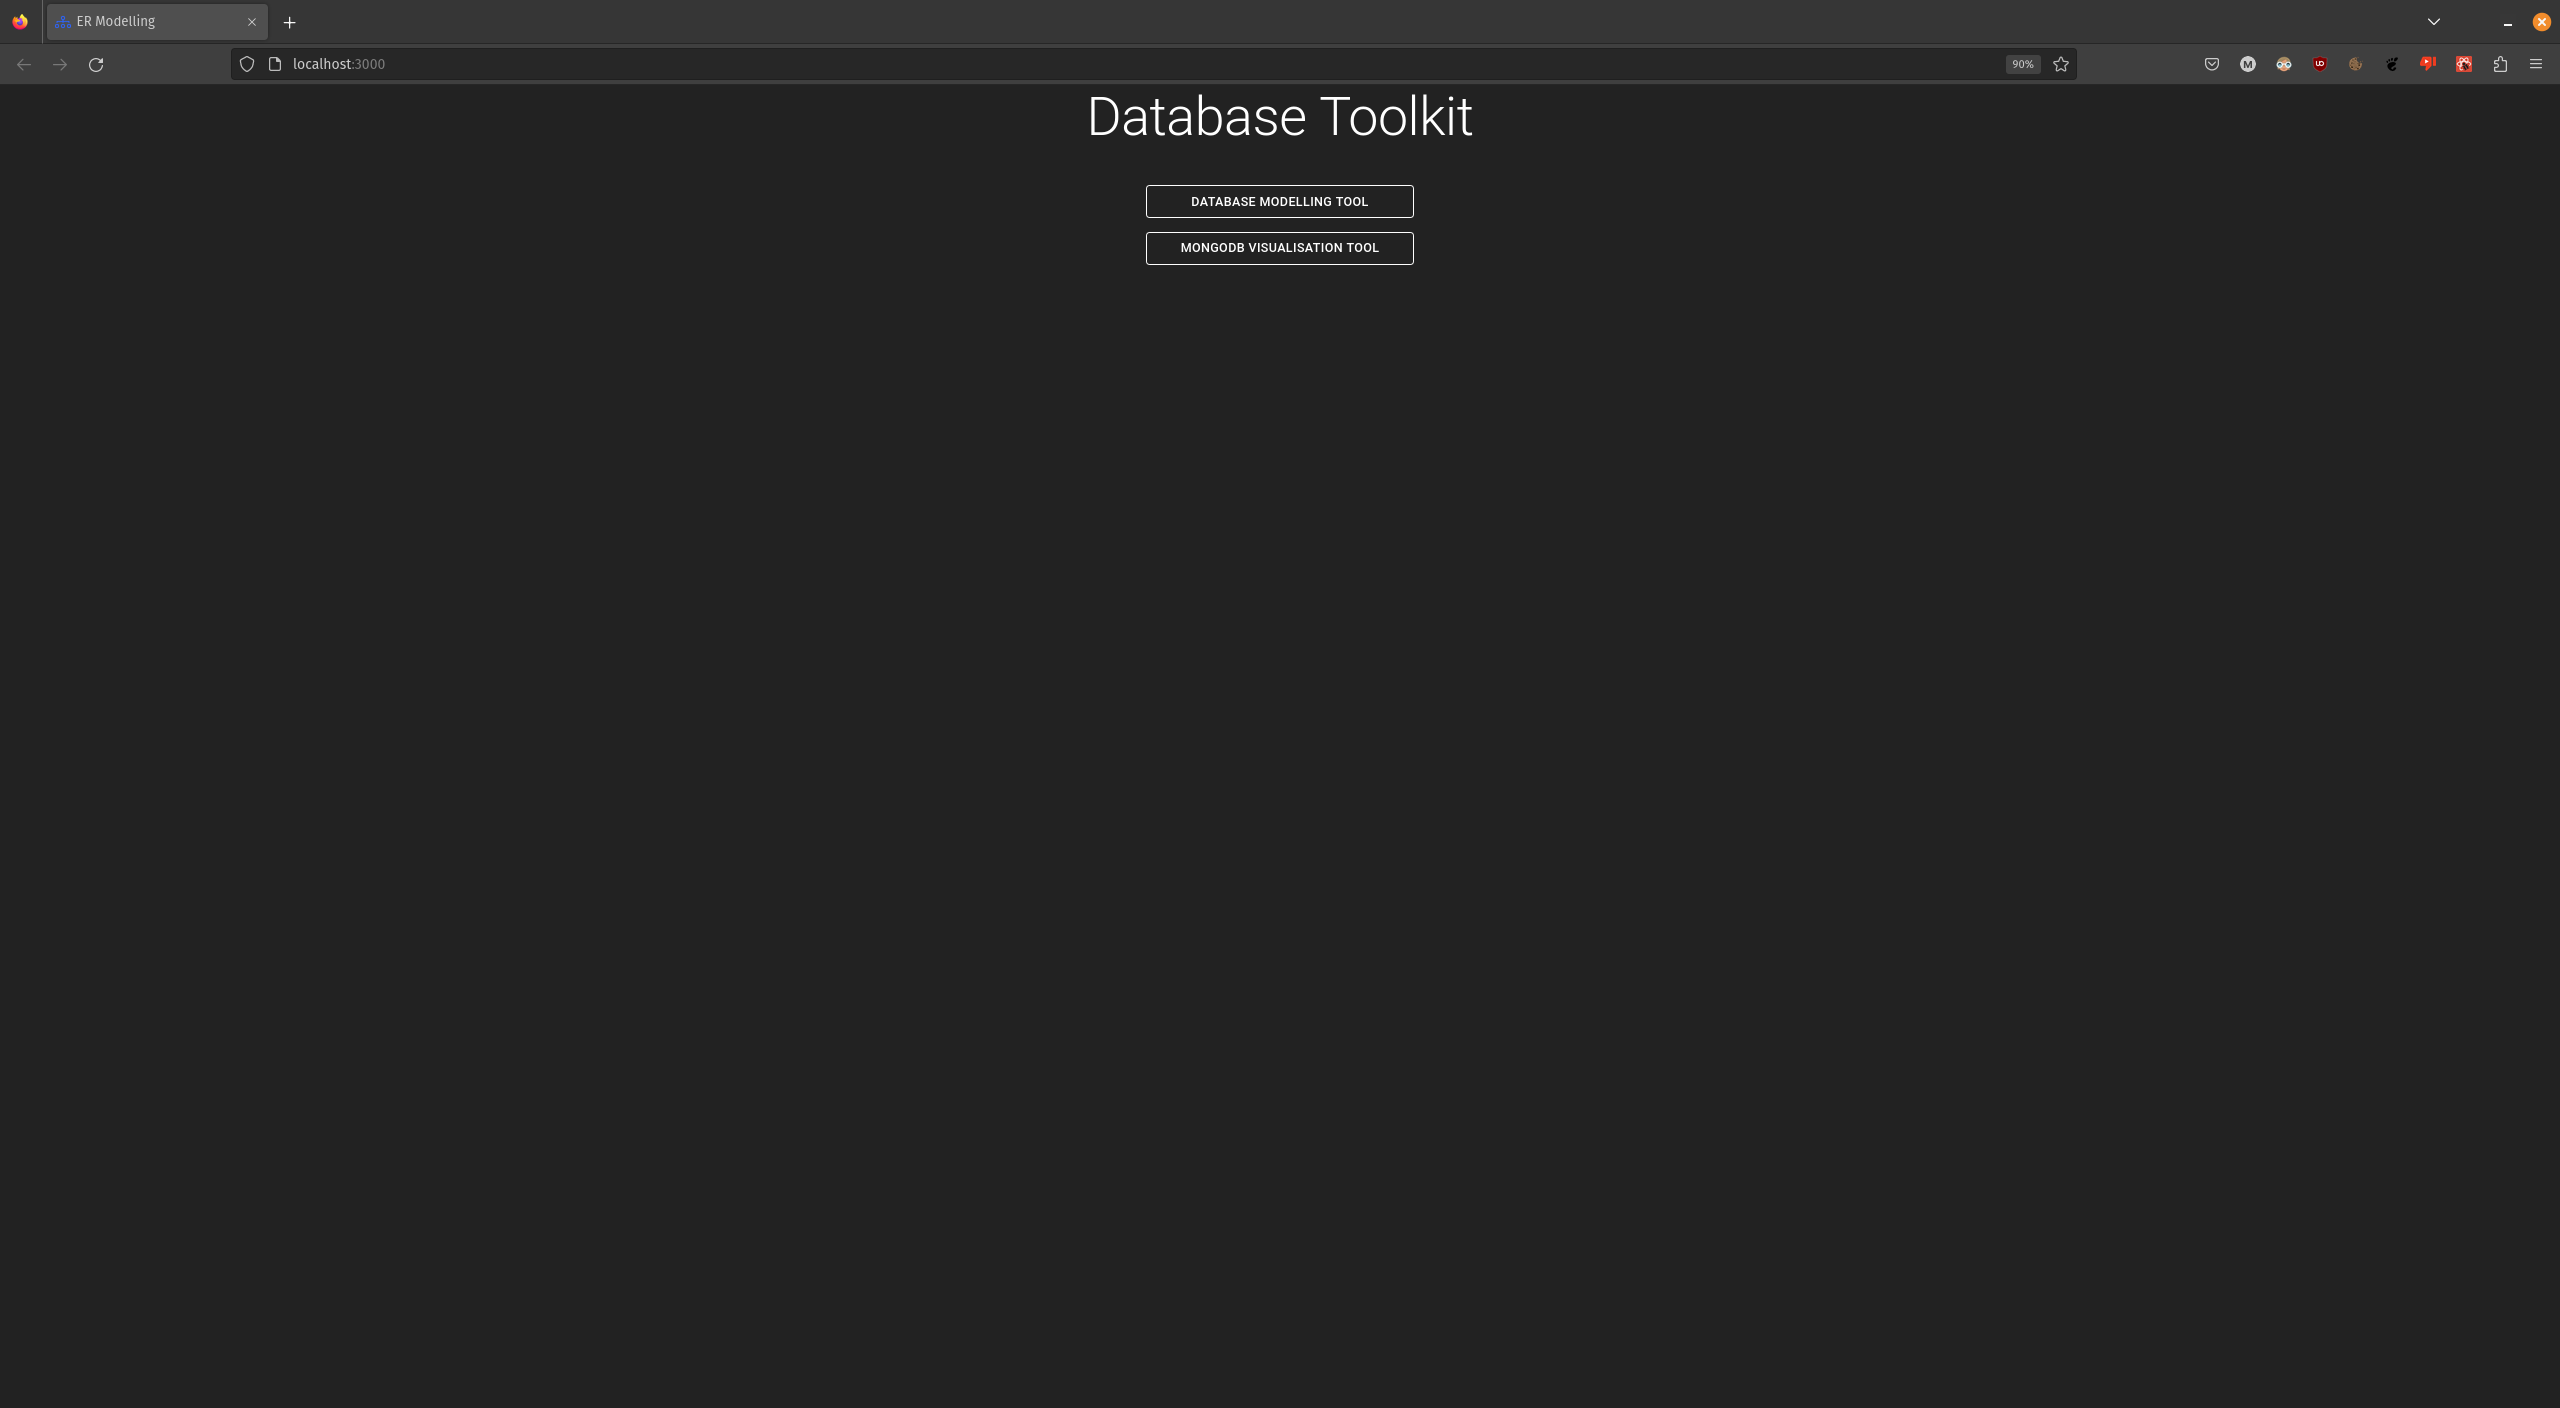
\includegraphics[width=\textwidth]{images/frontend_titlescreen}
    \caption{Frontend Startbildschrim}
    \label{fig:frontend_titlescreen}
\end{figure}

Das Rendern der einzelnen Tool Screens erfolgt daraufhin in der Datei App.js.
Hier wird mittels React Router der Startbildschirm als Index Element definiert, welches initial angezeigt wird.
Zudem wird der Pfad aller weiteren Screens definiert, über welchen diese dann geladen werden können.

\begin{lstlisting}[language=JavaScript, caption={React Router in App.js},label={lst:app.js}]
<BrowserRouter>
    <Routes>
        <Route index element={<TitleScreen/>}/>
        <Route path={AppScreens.dbModellingTool} element={<DatabaseModellingTool/>}/>
        <Route path={AppScreens.mongoVisTool} element={<MongoManager/>}/>
    </Routes>
</BrowserRouter>
\end{lstlisting}

\subsection{Aufbau des MongoDB Visualisation Tool Frontends}
\label{sub:fe_aufbau}
Das oberste Element des MongoDB Visualization Tools ist der MongoManager, welcher die MongoLeftSidebar und das MongoDiagram enthält.
Mithilfe der MongoLeftSideBar kann die Verbindung und Analyse der MongoDB Datenbank konfiguriert und durchgeführt werden.
Nach dem Verbinden und Analysieren werden in dem MongoDiagram DocumentTables angezeigt, welche rekursiv geschachtelt wieder DocumentTables enthalten können.
Darüber hinaus gibt es noch ein DetailView Popup, welches angezeigt wird, wenn man auf den Titel eines DocumentTables klickt.
Die DetailView enthält ebenfalls DocumentTables, welche auch wieder rekursiv geschachtelt sein können.
(Das DetailView Popup ist in der nachfolgenden Grafik nicht abgebildet)

\begin{figure}[H]
    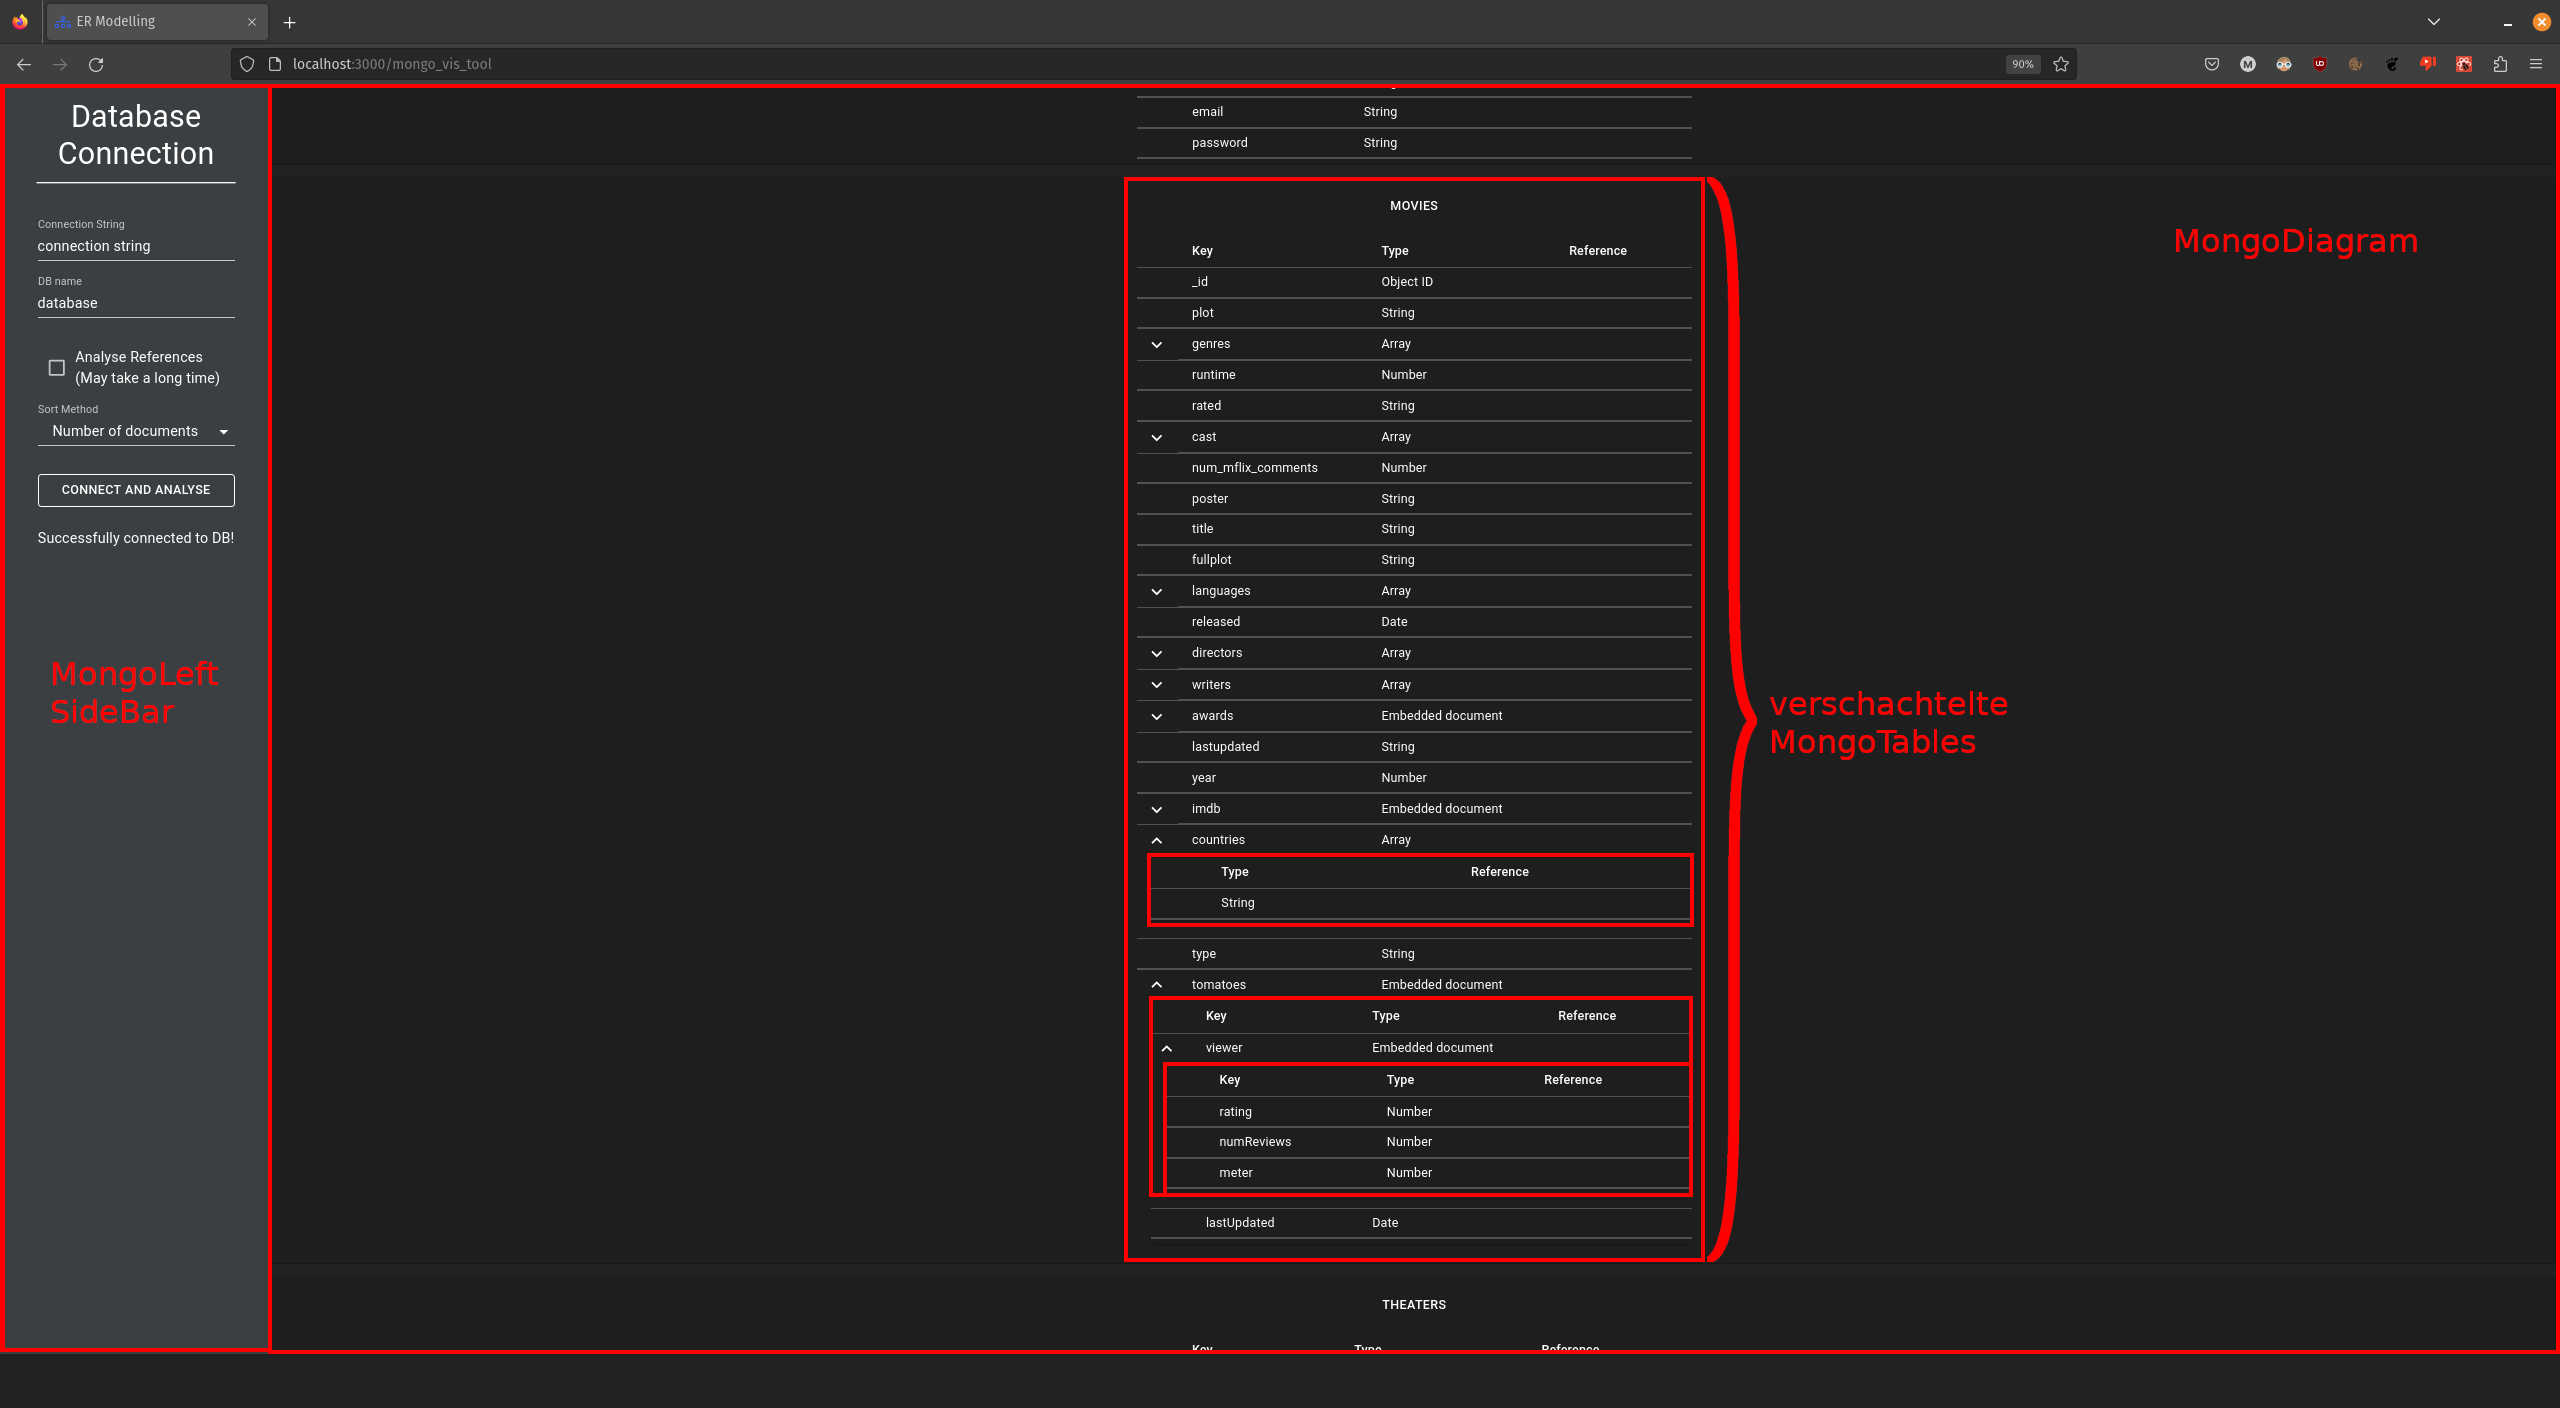
\includegraphics[width=\textwidth]{images/frontend_layers}
    \caption{Frontend Elemente}
    \label{fig:frontend_layers}
\end{figure}

\subsection{Left Sidebar}
\label{sub:fe_left_sidebar}

Die  MongoLeftSideBar nutzt die Material UI Komponenten Typography, TextField, FormControl und Button, um das Eingeben der Verbindungs- und Analysedetails zu ermöglichen.
Diese Informationen werden bei jeder Änderung im State der MongoLeftSideBar gespeichert.
Nach dem Drücken des Connect-Buttons wird die Methode connectToDB aufgerufen.
In dieser Methode wird mit den im State gespeicherten Informationen mithilfe von Axios ein HTTP Request an das Backend gesendet.
Wenn die Verbindung erfolgreich ist, wird die Methode connectionSuccessful aufgerufen.
In dieser werden die analysierten Daten des Backends im ReduxStore gespeichert.
Dies löst im Anschluss das Rendering der DocumentTables im MongoDiagram aus.
Zudem wird das Feedback Label in der MongoLeftSideBar aktualisiert.
Im Fehlerfall wird nur das Feedback Label in der Methode connectionFailed aktualisiert.


%TODO url als Umgebungsvariable abfragen
\begin{lstlisting}[language=JavaScript, caption={MongoLeftSideBar.connectToDB},label={lst:mongo_left_side_bar_connect_to_db}]
function connectToDB() {
    console.log("connecting to db")
    setConnectionState(ConnectionStates.connecting)
    const url = "http://127.0.0.1:5000/connect"

    let contentToSend = {
        connection_string: connectionString,
        database: dbName,
        analyse_ref: analyseRef,
        sort_method: sortMethod
    };

    axios.post(url, contentToSend).then((response) => {
        connectionSuccessful(response)
    }).catch(error => connectionFailed(error))
}

function connectionSuccessful(response) {
    console.log("data: " + response.data)
    setConnectionState(ConnectionStates.connected)
    dispatch(setCollections(response.data))
}

function connectionFailed(error) {
    console.log(error)
    setConnectionState(ConnectionStates.connectionFailed)
}
\end{lstlisting}

\subsection{DocumentTable}
\label{sub:fe_document_table}

Ein DocumentTable repräsentiert ein Schema von Dokumenten in einer Collection.
Es gibt mehrere Arten von DocumentTables, welche je nach Verwendungszweck mit dem Enum DocumentTableType unterschieden werden:
\begin{itemize}
    \item \textbf{main} ist die standard Tabelle, welche im MongoDiagram benutzt wird, um das Hauptschema einer Collection darzustellen.
    \item \textbf{nested} ist eine veschachtelte Untertabelle, entspricht also dem Datentyp Embedded Document.
    \item \textbf{array} wird für den Datentyp Array benutzt.
    \item \textbf{detail} wird im DetailView Popup benutzt, um alle Variatonen der Schemas einer Collection darzustellen.
\end{itemize}

Dem Element DocumentTable liegt die Material UI Table zugrunde.
Material UI Tables haben eine Toolbar, welche hierfür je nach DocumentTableType angepasst wird.
In der Main DocumentTable besteht die Toolbar aus einem Button, mit dem Namen der dargestellten Collection als Label.
Die onClick Methode dieses Buttons öffnet die DetailView dieser Collection.
Wenn der DocumentTableType detail entspricht, zeigt die Toolbar die Anzahl der Dokumente, die dieses Schema benutzen, sowie eventuell die fehlenden Felder gegenüber dem Hauptschema.
In allen anderen Fällen bleibt die Toolbar leer.

Die Spaltenüberschriften im Tablehead sind <Leer> - Key - Type - Reference.
Wenn es sich um ein Array Handelt, wird die Spalte Key weggelassen.
Die Reihen selbst haben in der ersten Spalte entweder einen Expand Button, mit dem sich Untertabellen und Arrays ausklappen lassen, oder nichts.
In den nachfolgenden Spalten werden die Daten aus dem Backend eingefüllt.
Nach jeder Reihe folgt eine zunächst unsichtbare Reihe.
Wenn der Datentyp des Werts in dieser Reihe Array oder Embedded document entspricht, wird in dieser unsichtbaren Reihe die entsprechende Untertabelle geladen.
Diese lässt sich dann mit dem Expand Button ausklappen und anzeigen.

\begin{figure}[H]
    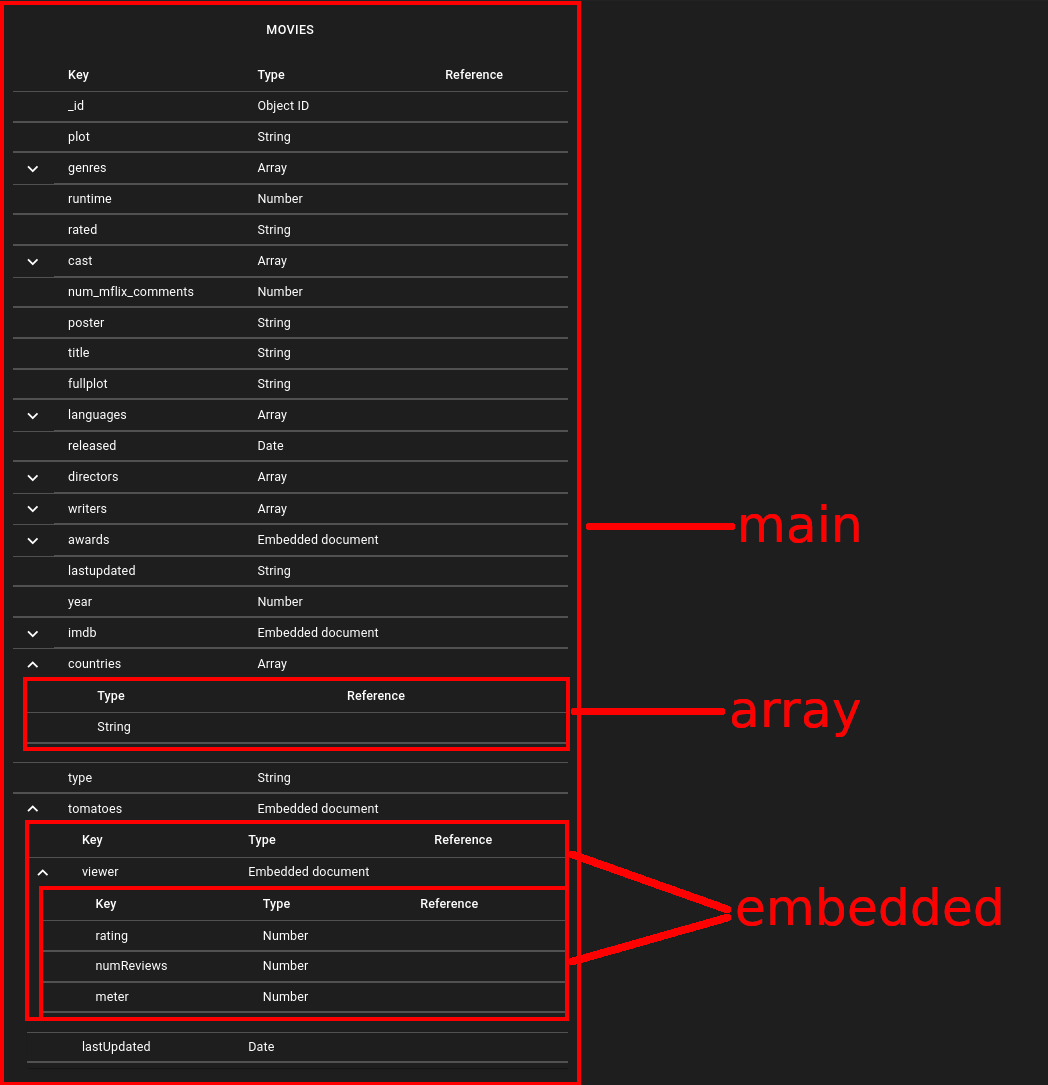
\includegraphics[width=360pt]{images/table_types}
    \caption{Frontend DocumentTable Typen}
    \label{fig:table_types}
\end{figure}

\subsection{DetailView Popup}
\label{sub:fe_detail_view}

Tatsächlich rendert die return Methode des DetailViewPopups zunächst nur einen Button. 
Erst wenn dieser Button gedrückt wird, wird das Popup als Material UI Modal angezeigt.
Dieses Modal lädt daraufhin, wie auch der MongoManager, DocumentTables.
Der DocumentTableType ist in diesen Tabellen jedoch nicht main, sondern detail, was die Toolbars der Tabellen verändert.


\begin{figure}[H]
    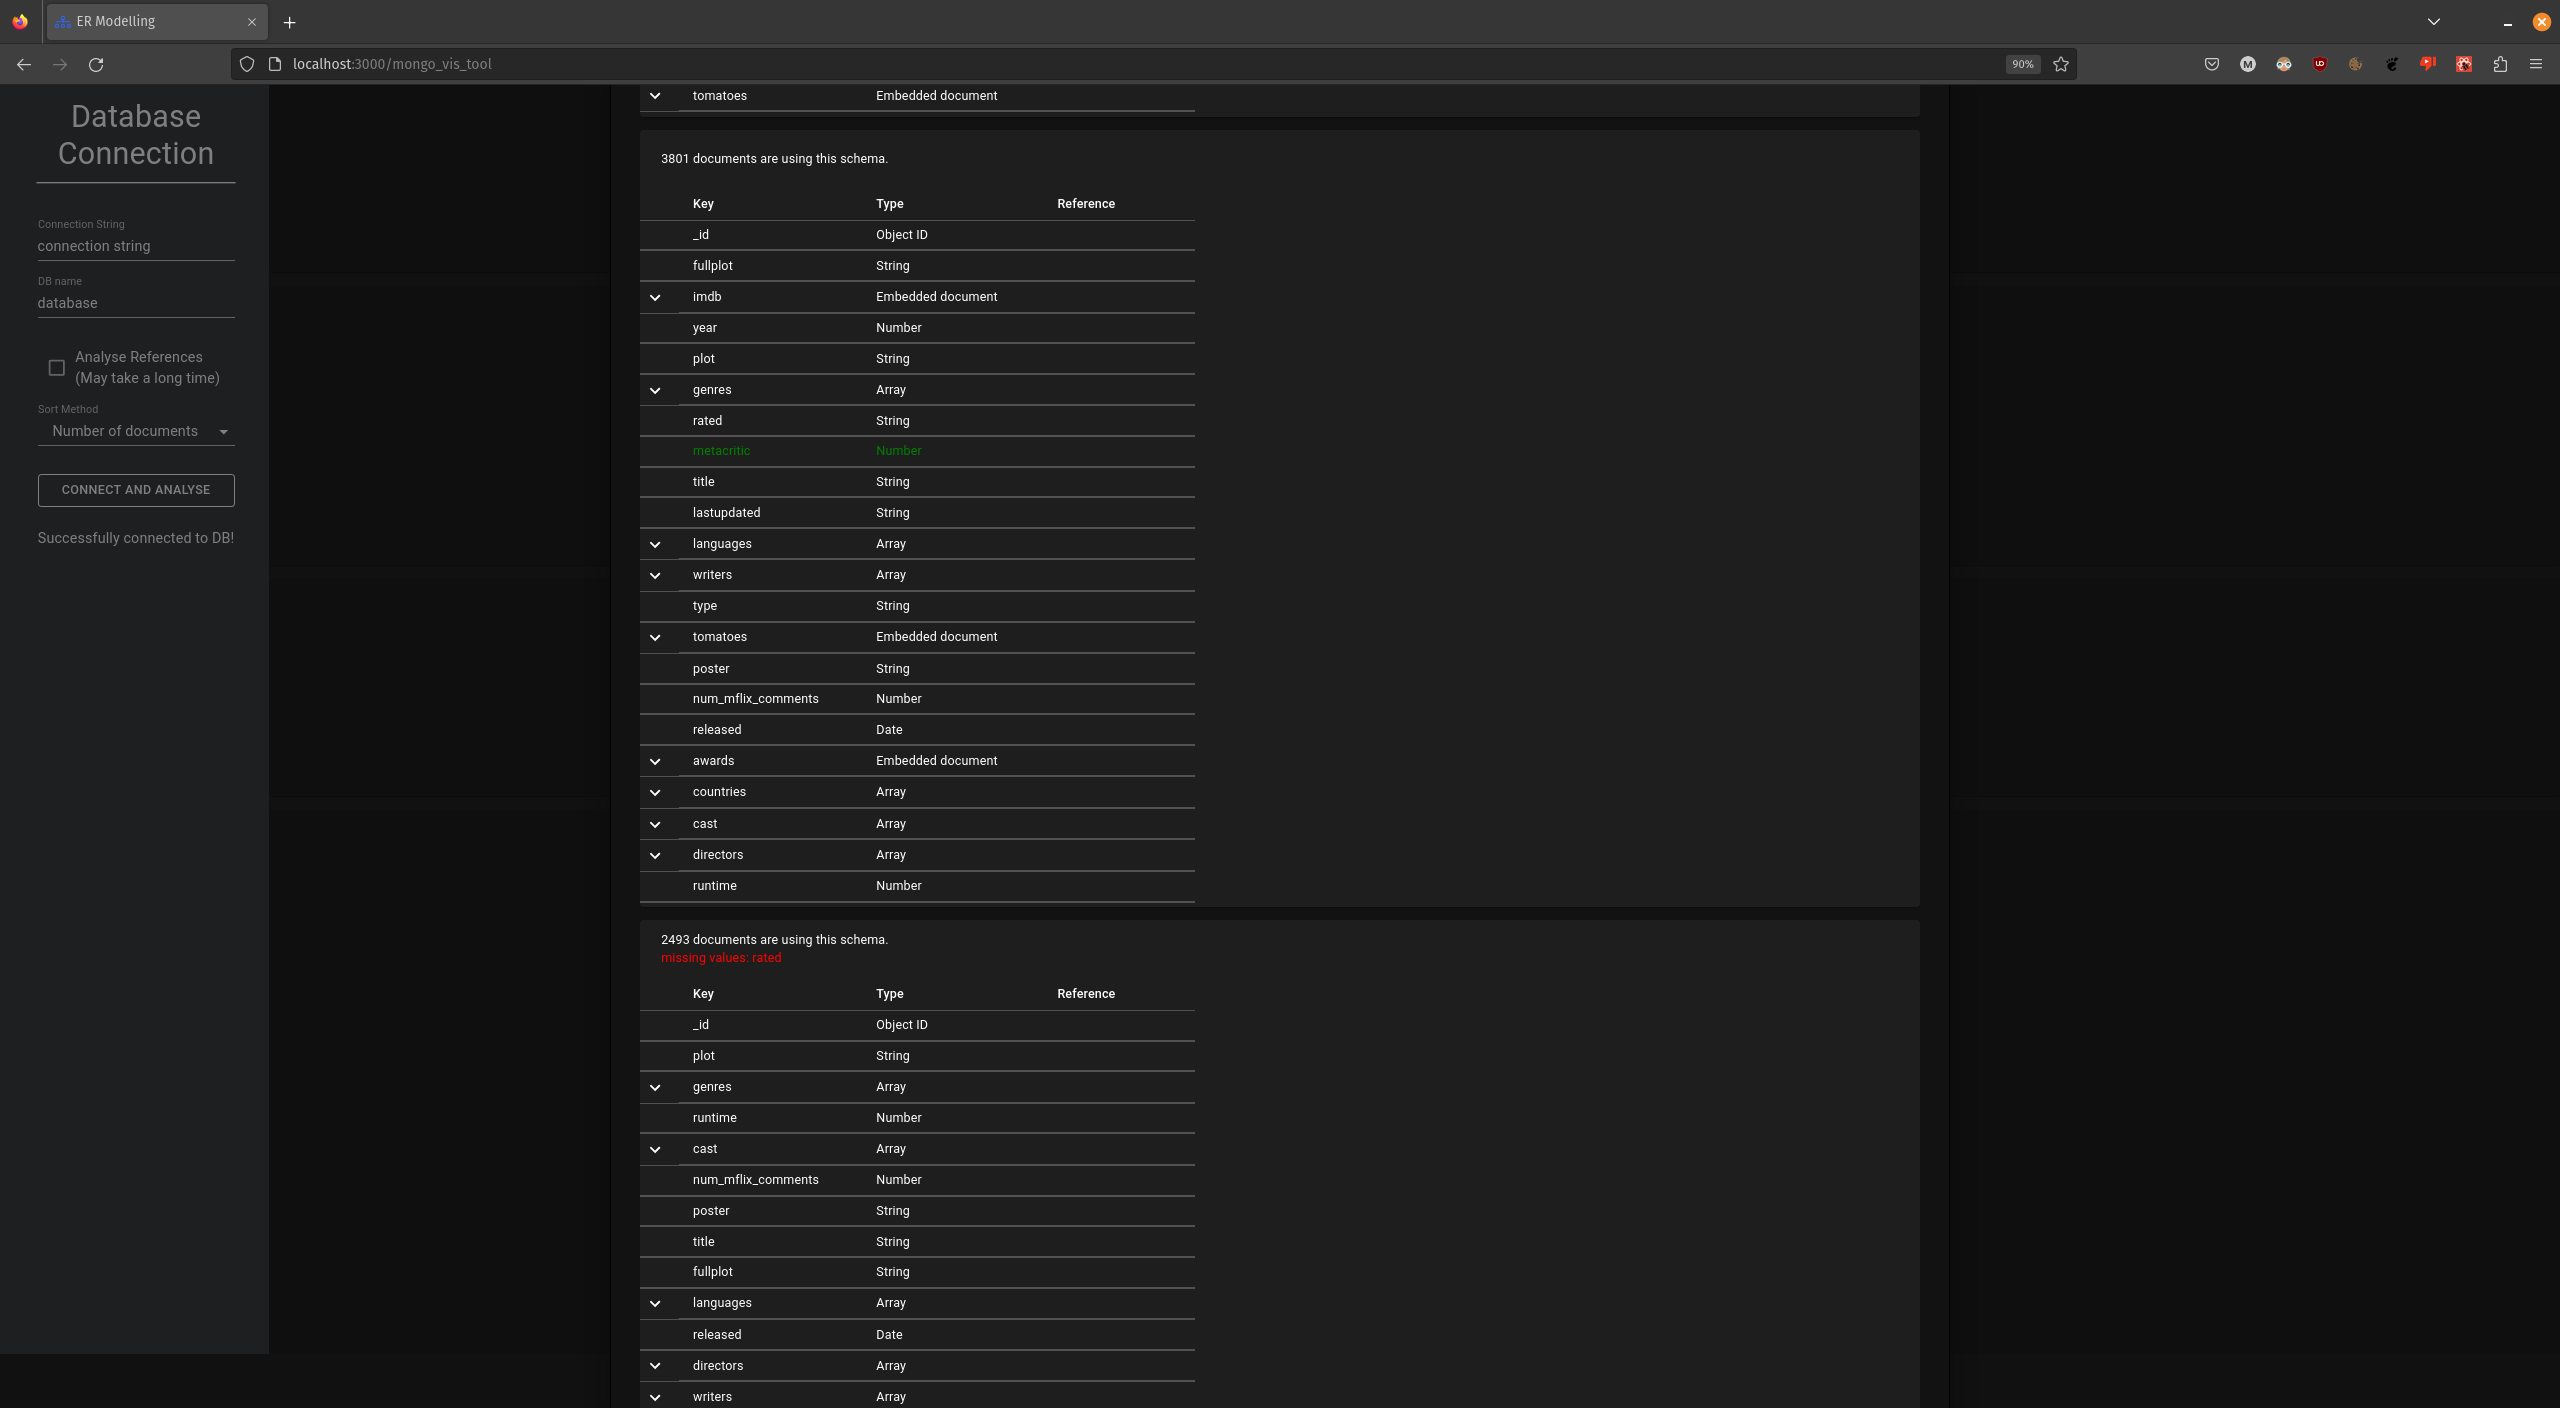
\includegraphics[width=\textwidth]{images/frontend_detail_view}
    \caption{Frontend DetailView Popup}
    \label{fig:frontend_detail_view}
\end{figure}

\subsection{Redux Store}
\label{sub:fe_redux}

Der Redux Store dient dem Speichern von States losgelöst von einzelnen React Komponenten.
Für das Speichern eines States wird ein sogenannter ContentSlice verwendet.
Die ContentSlices für das MongoDB Visualisierungstool sind alle grundsätzlich gleich aufgebaut:
Im initialState wird der Ausgangszustand des States definiert. 
Im Fall des MongoContentSlice wird initial collections auf null gesetzt.
Reducer sind Methoden, welche das Beschreiben des States erlauben.
in diesem Fall wurde der Reducer setCollections definiert, welcher es erlaubt, in collections das Argument documents zu schreiben.
Abschließend werden die actions und die reducer des ContentSlice exportiert, sodass diese global erreichbar sind.

\begin{lstlisting}[language=JavaScript, caption={MongoContentSlice},label={lst:fe_redux_slice}]
export const mongoContentSlice = createSlice({
    name: 'mongoContent',
    initialState: {
        collections: null
    },
    reducers: {
        setCollections: (state, documents) => {
            state.collections = documents
        }
    }
})

export const {setCollections} = mongoContentSlice.actions
export default mongoContentSlice.reducer
\end{lstlisting}

Auf diese Weise lassen sich schnell und einfach weitere ContentSlices definieren.
Um die ContentSlices zu verwenden, müssen diese nur noch in den Redux Store eingefügt werden.

\begin{lstlisting}[language=JavaScript, caption={Redux Store},label={lst:fe_redux_store}]
export const store = configureStore({
    reducer: {
        erContent: erContentSlice,
        relationalContent: relationalContentSlice,
        mongoContent: mongoContentSlice
    }
})

export default store;
\end{lstlisting}


%---
\chapter{Inbetriebnahme}
\label{cha:inbetriebnahme}
\iffalse
Aufgabe des Kapitels Inbetriebnahme ist es, die Überführung der in 
Kapitel \ref{cha:implementierung} entwickelte Lösung in das betriebliche 
Umfeld aufzuzeigen. Dabei wird beispielsweise die Inbetriebnahme eines 
Programms beschrieben oder die Integration eines erstellten 
Programmodules dargestellt.

Bei der Software-Erstellung entspricht dieses Kapitel der 
Auslieferungsphase (Deployment) im \ac{rup}.
\fi

Das MongoDB Visualisation Tool wird auf einem Linux Server mit Debian 11 gehostet.
Das Flask Backend läuft in einem Docker Container.
Der Vorteil von Docker ist, dass der Applikation eine eigene Umgebung bereitgestellt wird, die unabhängig vom Host-System ist.
Um das Backend als Dockercontainer auszuliefern, wurde das vorkonfigurierte Docker Image uwsgi-nginx-flask von tiangolo genutzt.
In diesem Docker Image sind uWSGI und Nginx vorinstalliert, was das Ausliefern von Flask Applikationen erleichtert.
~\autocite{tiangolo:uwsgi-nginx-flask}

Das Backend für das ER Modelling Tool ist als Heroku-App deployed.
Heroku ist ein cloudbasierter Serviceanbieter, welcher ein kostenloses Modell für das Hosting von Software und DNS anbietet.
~\autocite{heroku:heroku}

Das Frontend wurde mittels NPM gebaut und auf dem Server bereitgestellt.
Mittels NGINX wurde das Webinterface daraufhin gehostet. 
Das Interface ist nun unter der Adresse \url{https://db-toolkit.kodewisch.com} erreichbar.

\section{Buildprozess des Backends}
\label{sec:build_backend}

Um das Backend starten zu können, muss Python 3.10 oder neuer installiert sein.

Wenn dies der Fall ist, können mit dem Befehl \lstinline{pip -r requirements.txt} im Verzeichnis mongo\_vis\_backend alle benötigten Pakete installiert werden.
Um Konflikte mit anderen Python Installationen zu vermeiden, führt man diesen Befehl am besten in einem Virtual Environment aus.
Anschließend kann das Backend mit dem Befehl \lstinline{python3 -m flask run} ausgeführt werden.

Eine Anleitung für das Deployment des Backends als Docker Container kann unter \url{https://hub.docker.com/r/tiangolo/uwsgi-nginx-flask/} gefunden werden.

\section{Buildprozess des Frontends}
\label{sec:build_frontend}

Node und NPM müssen installiert sein, damit das Frontend gebaut werden kann.
Über \url{https://nodejs.org/en/download/} können Node und NPM installiert werden.

Anschließend müssen im Verzeichnis frontend folgende Befehle ausgeführt werden, um das Frontend zu starten:

\begin{lstlisting}[language=bash, caption={Frontend build commands},label={lst:fe_build_commands}]
$ npm install
$ npm start
\end{lstlisting}    

Um das Frontend auszuliefern, kann das Frontend mit dem Befehl \lstinline{npm run build} gebaut werden.
Die gebauten Dateien befinden sich dann im Ordner build.

Vorausgesetzt wird ein Debian- oder Ubuntubasierter Computer oder Server, auf dem Nginx mit SSL-Zertifikat konfiguriert ist.
Um die Dateien auf solch einem Server auszuliefern, müssen die Dateien in den Ordner /var/www/db-toolkit/html verschoben werden.
Der Ordnername db-toolkit kann auch durch einen beliebigen anderen Namen ersetzt werden.
Daraufhin muss folgende Nginx Konfiguration im Ordner /etx/nginx/conf.d mit dem namen db-toolkit.conf angelegt werden:

\begin{lstlisting}[language=bash, caption={db-toolkit.conf},label={lst:db-toolkit.conf}]
server { 
    listen 80; 
    listen [::]:80; 
    server_name db-toolkit.kodewisch.com; 
    return 301 https://$host$request_uri; 
} 

server { 
    listen 443 ssl; 
    server_name db-toolkit.kodewisch.com;

    ssl_certificate /etc/letsencrypt/live/kodewisch.com/fullchain.pem; 
    ssl_certificate_key /etc/letsencrypt/live/kodewisch.com/privkey.pem; 
    include /etc/letsencrypt/options-ssl-nginx.conf; 
    ssl_dhparam /etc/letsencrypt/ssl-dhparams.pem; 

    root /var/www/db-toolkit/html;
    index index.html index.htm;

    location / { 
        try_files $uri $uri/ =404; 
    } 
}
\end{lstlisting}    

Diese Nginx Konfiguration zeigt die unter root und index spezifizierte Resource für alle Anfragen an, die auf die Subdomain db-toolkit.kodewisch.com eingehen.
Die obere Server-Konfiguration nimmt die HTTP Anfragen auf Port 80 entgegen und leitet diese auf HTTPS um.
Die untere Server-Konfiguration nimmt die HTTPS Anfragen auf Port 443 entgegen, spezifiziert das SSL-Zertifikat und zeigt die Resource an.
Die ssl\_certificate Pfade müssen durch die entsprechenden Pfade auf dem Server ersetzt werden, ebenso wie die Domain.


%---
\chapter{Evaluierung}
\label{cha:evaluierung}

Aufgabe des Kapitels Evaluierung ist es, in wie weit die Ziele der 
Arbeit erreicht wurden. Es sollen also die erreichten Arbeitsergebnisse 
mit den Zielen verglichen werden. Ergebnis der Evaluierung kann auch 
sein, das bestimmte Ziele nicht erreicht werden konnten, wobei die 
Ursachen hierfür auch außerhalb des Verantwortungsbereichs des 
Praktikanten liegen können.

%---
\chapter{Zusammenfassung und Ausblick}
\label{cha:zusammenfassung}
\section{Erreichte Ergebnisse}
\label{sec:ergebnisse}

\iffalse
Die Zusammenfassung dient dazu, die wesentlichen Ergebnisse des 
Praktikums und vor allem die entwickelte Problemlösung und den 
erreichten Fortschritt darzustellen. (Sie haben Ihr Ziel erreicht und 
dies nachgewiesen).
\fi

In diesem Projekt wurde das Problem angegangen, dass es keine geeigneten Schema-Analysetools für MongoDB Datenbanken gibt.
Deshalb wurde das MongoDB Visualisierungstool entwickelt.
Dieses Tool wurde in das bestehende Projekt ER Modellierungstool integriert, um ein erweiterbares Datenbank Toolkit zu bilden.
Das Tool selbst besteht dabei aus 2 Teilen:
Der erste Teil ist ein Frontend, welches in das ER Modellierungstool Frontend integriert wurde.
Dieses Frontend wurde mit JavaScript und React umgesetzt.
Die Modularität dieser Gesamtlösung wurde durch einen Startbildschirm, sowie strukturelle Anpassungen im Code erweitert.
Das MongoDB Visualisierungstool Frontend besteht aus drei Hauptelementen:
\begin{itemize}
    \item Der LeftSidebar, die das Verbinden mit einer MongoDB Datenbank ermöglicht
    \item Dem MongoDiagram, welches einen Überblick über die meistverwendeten Schemas in den Collections gibt
    \item und dem DetailView Popup, welches alle Schemas in einer Collection anzeigt und die Unterschiede hervorhebt.
\end{itemize}

Die Schemas wurden hierbei mit der Komponente DokumentTable umgesetzt, welche auf der Material UI Table Komponente basiert.

Der zweite Teil des MongoDB Visualisierungstools ist ein Backend, welches in dem Python-Framework Flask geschrieben wurde.
Das Backend besitzt einen einzigen REST-Endpunkt.
Die Aufgabe dieses Endpunkts ist es, sich mit der spezifizierten Datenbank zu verbinden und diese zu analysieren.
Die Ergebnisse der Analyse werden an das Frontend im JSON-Format zurückgegeben, welches diese anschließend visualisert.

\section{Ausblick}
\label{sec:ausblick}

\iffalse
Im Ausblick werden Ideen für die Weiterentwicklung der erstellten Lösung 
aufgezeigt. Der Ausblick sollte daher zeigen, dass die Ergebnisse der 
Arbeit nicht nur für die in der Arbeit identifizierten Problemstellungen 
verwendbar sind, sondern darüber hinaus erweitert sowie auf andere 
Probleme übertragen werden können.
\fi

Es gibt ein Paar Funktionen des MongoDB Visualisierungstools, die noch weiter ausgebaut werden könnten.

\subsection{Referenzen}
\label{sub:ausblick_referenzen}

Einerseits erfolgt das Ermitteln der Referenzen noch nicht sehr präzise.
In dem aktuellen Algorithmus wird davon ausgegangen, dass alle Werte des Typs Object ID, welche nicht den Namen \_id besitzen, Referenzen sind.
Jedoch kann es auch Referenzen geben, die nicht den Typ Object ID besitzen, da der Primary Key eines Dokuments nicht zwangsläufig eine Object ID sein muss.
Deshalb könnte man die Bestimmung der Referenzen noch weiter verbessern.

Die Visualisierung der Referenzen könnte ebenfalls ausgebaut werden:
Man könnte eine Ansicht der Collections als Graph mit den Collections als Knoten und den Referenzen als Kanten darstellen.
Dies würde es Entwicklern bei Datenbanken mit vielen Referenzen erleichtern, die Abhängigkeiten zwischen den Collections zu überblicken.

\subsection{Performance der Analyse}
\label{sub:ausblick_performance}

Wie in dem Experiment im Kapitel \nameref{cha:evaluierung} festgestellt wurde, kann die Analyse von großen Datenbanken lange dauern.
Die Analyse der größten Datenbank im Experiment dauerte 30 Sekunden.
Solch eine lange Wartezeit unterbricht den Arbeitsablauf eines Entwicklers und sollte deswegen möglichst vermieden werden.
Dafür gibt es mehrere Ansätze:

Mittels Multithreading kann die Analysezeit erheblich reduziert werden.
Beispielsweise kann jede Collection auf einem eigenen Thread analysiert werden.
Da das Backend in Python geschrieben ist, ist die Umsetzung von Multithreading relativ simpel.
Python bietet mit der Bibliothek MultiProcessing eine simple, aber effiziente Implementierung von Multithreading an.
~\autocite{python:multiprocessing}

Eine weitere Möglichkeit, die Laufzeit der Analyse zu senken, ist, in größeren Datenbanken optional nur einen Teil der Dokumente jeder Collection zu analysieren.
Damit kann die Laufzeit linear gesenkt werden, abhängig von der Anzahl der nicht Dokumente, die nicht analysiert werden.
Jedoch ist es mit dieser Methode nicht mehr möglich, alle Schemavariationen einer Collection zuverlässig anzuzeigen.

Abgesehen von Software-Seitigen Optimierungen kann die Laufzeit verbessert werden, in dem man das Backend auf einem leistungsstärkeren Server ausliefert.

\subsection{Weitere Datenbanksysteme}
\label{sub:ausblick_weitere_dbs}

Neben MongoDB gibt es noch eine Vielzahl weiterer Datenbanksysteme, für welche keine geeigneten Visualisierungstools existieren.
Man kann das MongoDB Visualisierungstool beispielsweise zu einem NoSQL Visualisierungstool erweitern.
Vorstellbar wäre eine Einstellung in der LeftSideBar, in der man den Typ der zu analysierenden Datenbank auswählen kann.
Mit dieser Information kann man daraufhin in der MongoDiagram Komponente eine passende Visualisierung anzeigen.
Vor allem für Dokument-Datenbanken und andere zu MongoDB ähnliche Datenbanken wäre der Aufwand, diese zu integrieren, gering, da die nötigen Komponenten zur Visualisierung dieser bereits existieren und lediglich angepasst werden müssten.
Aber auch andere NoSQL Datenbanken, wie beispielsweise Graph-Datenbanken, könnten in das Visualisierungstool integriert werden.

\subsection{Weitere Tools}
\label{sub:ausblick_tools}

Neben den zwei bestehenden Tools kann das Datenbank Toolkit um weitere Tools erweitert werden.
Das Datenbank Toolkit ist entsprechend modular aufgebaut, sodass weitere Tools ohne große Änderungen in das bestehende Toolkit integriert werden können.


%-----------------------------------------------------------------------
\appendix

%---
\printbibliography[heading=bibintoc]

%---
\chapter{Anhang A}

%---
\chapter{Anhang B}


\end{document}
